\documentclass{padalreport}

\usepackage{rotating}
\usepackage{textcomp}

% \usepackage{tikz}
\usepackage{xspace}
\usepackage{todonotes}
\usepackage{setspace}

% modern bibliography management
\usepackage[backend=biber,style=numeric,sorting=nyt,hyperref,defernumbers=true,maxcitenames=4,mincitenames=4,maxbibnames=100,firstinits=true]{biblatex}


\addbibresource[label=primary]{references.bib}

%\usepackage{draftwatermark}
%\SetWatermarkText{DRAFT}
%\SetWatermarkScale{2}

\setcounter{tocdepth}{3}

\usepackage{amsmath, amsthm, amssymb}

\usepackage[pdftex,bookmarksopen,bookmarksnumbered,linkcolor=black,citecolor=black,urlcolor=black]{hyperref}

\usepackage{subfigure}

%\usepackage{draftwatermark}
%\SetWatermarkScale{1}

\usepackage{multirow}
\usepackage{colortbl}

\usepackage{float}
\newfloat{program}{htbp}{lop}
\floatname{program}{Code}

\usepackage{dblfloatfix}

\setcounter{tocdepth}{3}

\usepackage{float}




\PADALtitle{Programming Abstractions for Data Locality}



\date{}           % Leave this here but empty

%\PADALauthor{
%author list goes here
%}
%
%\PADALauthorshort{
%author list goes here
%}

\pagestyle{empty}
\phantomsection
%\addcontentsline{toc}{section}{Abstract}
%\pdfbookmark{1}{Abstract}{Abstract}
\begin{center}
\vspace{2em}
{\bf \huge Programming Abstractions for Data Locality
}\\[\baselineskip] % d. Proposal title \vspace{2em}

{\em April 28 -- 29, 2014 \\
Swiss National Supercomputing Center (CSCS), Lugano, Switzerland} \\
\end{center}

\noindent
\textbf{Co-Chairs}\\
\noindent
Didem Unat (LBNL)\\
Torsten Hoefler (ETH Z{\"u}rich) \\
John Shalf (LBNL) \\
Thomas Schulthess (CSCS) \\

\begin{center}
\noindent
\textbf{Workshop Participants/Co-Authors} \\
\end{center}
\begin{multicols}{2}

% Perhaps identify section leads using asterisk and footnotes, or in separate column?
\noindent
{\small
Adrian Tate (Cray) \\
Amir Kamil (Lawrence Berkeley National Laboratory)\\
Anshu Dubey (Lawrence Berkeley National Laboratory)\\
Armin Gr��linger (University of Passau)\\
Brad Chamberlain (Cray)\\
Carter Edwards (Sandia National Laboratories)\\
Chris J. Newburn (Intel)\\
David Padua (UIUC)\\
Didem Unat (Lawrence Berkeley National Laboratory)\\
Emmanuel Jeannot (INRIA) \\
Frank Hannig (University of Erlangen-Nuremberg)\\
Gysi Tobias (ETH Z{\"u}rich)\\
Hatem Ltaief (KAUST)\\
James Sexton (IBM)\\
Jesus Labarta (Barcelona Supercomputing Center)\\
John Shalf (Lawrence Berkeley National Laboratory)\\
Karl Fuehrlinger (Ludwig-Maximilians-University)\\
Kathryn O'Brien (IBM)\\
Leonidas Linardakis (Max Planck Inst. for Meteorology)\\
Maciej Besta (ETH Z{\"u}rich)\\
Marie-Christine Sawley (Intel, Europe)\\
Mark Abraham (KTH)\\
Mauro Bianco (CSCS)\\
Miquel Pericas (Chalmers University of Technology)\\
Naoya Maruyama (RIKEN)\\
Paul Kelly (Imperial College)\\
Peter Messmer (Nvidia)\\
Romain Cledat (Intel)\\
Satoshi Matsuoka (Tokyo Institute of Technology)\\
Thomas Schulthess (CSCS)\\
Torsten Hoefler (ETH Z{\"u}rich)\\
Vitus Leung (Sandia National Laboratories)\\
} \\
\end{multicols}
\noindent
\begin{center}
\textbf{Executive Summary}
\end{center}
{\small
The cost of data movement has become the dominant factor of a high performance computing system both in terms of energy consumption and performance. To minimize data movement, applications have to be optimized both for vertical data movement in the memory hierarchy and horizontal data movement between processing units. While microarchitectural technology trends allow the scaling of the number of cores per chip, cache coherence  will likely not scale to the large number of cores due to the traffic overhead of maintaining coherence. 
%In the future, software-managed memory and incoherent caches or scratchpad memory will be prevalent. Thus, application developers need a set of programming abstractions to describe data locality for the new computing ecosystem.
Architectural trends break our existing programming paradigm because the current software tools optimize for floating point operations not memory traffic. They ignore the incurred cost of communication and simply rely on the hardware cache coherency to virtualize data movement. For example, the current OpenMP-3 usage model describes how to parallelize loop iterations and divides the iteration space evenly among processors with limited flexibility for expressing data layout.  
% It implicitly assumes all the processing elements are equidistant to each other and equidistant to main memory. This does not reflect the underlying machine architecture. 
Application developers need a set of programming abstractions to describe data locality for the new computing ecosystem.
The new programming paradigm should be more data centric and allow to describe how to decompose and how to layout data in the memory.

Fortunately, there are many emerging concepts such as {\em tiling}, {\em array views} and {\em iterators} to managing data locality. There is an opportunity to identify commonalities in strategy to enable us to combine together the best of these concepts to develop a comprehensive approach to expressing and managing data locality on exascale programming systems. These programming model abstractions can expose crucial information about data locality to the compiler and runtime system to enable performance-portable code. The research question is to identify the right level of abstraction, which includes techniques that range from template libraries all the way to language constructs to achieve this goal.

\textbf{\em The goal of the workshop and this report is to identify common themes and standardize concepts for locality-preserving abstractions for exsacale programming models.}
}

\pagebreak
%
%Adrian Tate (Cray) 
%Amir Kamil (Lawrence Berkeley National Laboratory)
%Anshu Dubey (Lawrence Berkeley National Laboratory)
%Armin Gr��linger (University of Passau)
%Brad Chamberlain (Cray)
%Carter Edwards (Sandia National Laboratories)
%Chris J. Newburn (Intel)
%David Padua (UIUC)
%Didem Unat (Lawrence Berkeley National Laboratory)
%Emmanuel Jeannot (INRIA) 
%Frank Hannig (University of Erlangen-Nuremberg)
%Gysi Tobias (ETH Z�rich)
%Hatem Ltaief (KAUST)
%James Sexton (IBM)
%Jesus Labarta (BSC)
%John Shalf (Lawrence Berkeley National Laboratory)
%Karl Fuehrlinger (Ludwig-Maximilians-University, M�nchen )
%Kathryn O'Brien (IBM)
%Leonidas Linardakis (Max Planck Institute for Meteorology)
%Maciej Besta (ETH Z�rich)
%Marie-Christine Sawley (Intel, Europe)
%Mark Abraham (KTH)
%Mauro Bianco (CSCS)
%Miquel Pericas (Chalmers University of Technology)
%Naoya Maruyama (RIKEN)
%Paul Kelly (Imperial College)
%Peter Messmer (Nvidia)
%Romain Cledat (Intel)
%Satoshi Matsuoka (Tokyo Institute of Technology)
%Thomas Schulthess (CSCS)
%Torsten Hoefler (ETH Z�rich)
%Vitus Leung (Sandia National Laboratories)
%
%
%Session 1 - Applications 
%
%Memory Abstraction via Subsets in the ICON Domain Specific Language
%Leonidas Linardakis 
%Max Planck Institute for Meteorology
%
%Abstract: ICON is a next generation climate and weather prediction model, utilizing unstructured grids. Its memory layout, as well its access patterns, were originally designed for vector machines, which is suboptimal for cache-based machines. On the other hand, adapting large codes, like ICON, to new architectures is a tedious and error-prone process. We propose a memory abstraction scheme, in a form of a simple DSL extension, that allows the modelers to write their code in a way "natural" to the model, while at the same time provides the ability to adapt the memory layout and the access patterns to a given architecture.
%
%
%Increasing Productivity and Performance Portability through Domain-Specific Languages
%Frank Hannig 
%University of Erlangen - Nuremberg
%
%Abstract: Due to limited power budgets as well as the dark silicon phenomenon, the performance of computing systems will scale in the future only if energy efficiency will be improved significantly. Therefore, one trend is that systems become more and more heterogeneous and customized. The downside of this trend is the programmability of such complex systems, which requires either detailed knowledge of the specific architecture components or sophisticated compilers and runtime management. To cope with this programming challenge, we consider domain-specific approaches in order to automatically generate code for different architectures. More specific, I will present two approaches: The first one, HIPAcc (http://hipacc-lang.org), is a framework for designing image processing kernels in a domain-specific language (DSL) and subsequent generation of low-level target code for GPU accelerators by source-to-source translation. The second approach, ExaStencils (http://www.exastencils.org), targets stencil codes for exascale computing. Here, we currently develop a new software technology that is based on a multi-layered DSL, which forms the foundation for performance-portable refinement at different abstraction levels and allows for incorporation of techniques such as software product line engineering and polyhedral optimization.
%
%
%Exploration of Finer Computation Granularity Through Micro-blocking in AMR
%Anshu Dubey and Daniel T. Graves
%Lawrence Berkeley National Laboratory, USA
%
%Abstract: When using block structured adaptive mesh refinement (SAMR) with explicit numerical schemes a ?block? of discretized cells with surrounding ghost cells is the most common computational abstraction. The ?stencil? for updating each cell in the mesh determines the depth of ghost-cells layer and the memory overhead for each block. The fine-grain parallelism of newer HPC platforms makes smaller block sizes more attractive for better utilization of compute resources, but decreasing block sizes increases memory overheads. Therefore the ?block? abstraction is not very effective for fine-grain parallelism. However, if we separate the source and destination data containers for computing the state update of a block then it is possible to treat the source block as read-only. This allows blocks to be logically split into arbitrarily small ?micro-blocks? where the ghost cells of one micro- block overlap with the active cells of its neighboring micro-blocks in physical memory without any conflicts. No conflict arises in the destination data container either because there is no need for overlapped cells where updates are stored. We have implemented a prototype application with micro-blocking in Chombo to evaluate the potential of this abstraction in exploiting fine-grain parallelism of newer HPC platforms. We will present our findings from experiments using threading for fine-grain parallelism on various platforms.
%
%
%On the Need for Data Structures for Cache-aware Algorithms in GROMACS 
%Mark Abraham (KTH)
%
%Abstract: The authors of the high-performance molecular-dynamics simulation package GROMACS have identified problems in making best use of data locality in multi-core processors, despite the compute-bound parts of the code not leaving L2 cache. These problems will get worse in the exascale era. Solution constructs that do not require custom language features or compiler support are particularly important for highly portable code. I will show these problems and discuss how we think we can improve the situation with data structures that have more explicit awareness of the need to manage the side-effects of caches.
%
%Back to Schedule
%
%Session 2 - Data Structure and Layout Abstractions 
%
%An Overview of the DASH Project
%Karl Fuerlinger 
%Ludwig-Maximilians-University, M�nchen 
%
%Abstract: The DASH (Data Structures with Support for Hierarchical Locality) project develops a data-structure oriented C++ template library that provides hierarchical PGAS-like abstractions for various data containers (multidimensional arrays, lists, hash tables, etc.) and allows a developer to control (and explicitly take advantage of) the hierarchical data layout of global data structures. In contrast to other PGAS approaches, DASH does not propose a new language or require compiler support to realize global address space semantics. Instead, operator overloading and other C++ features are used to provide the semantics of data residing in a global and hierarchically partitioned address space based on a runtime system with one-sided messaging primitives provided by MPI or GASNet.
%
%
%Addressing Data Locality Challenge with Tiling Abstraction 
%Didem Unat and John Shalf 
%Lawrence Berkeley National Laboratory
%
%Abstract: Tiling, or blocking, is a well-known loop transformation to improve parallelism and data locality. Hardware trends towards massively parallel chips and mesh-like on-chip network topologies increase the importance of tiling transformations. As the data movement cost dominates both the energy consumption and performance, a programming model designed for exascale machines should take a data centric approach abstracting the hierarchy in memory subsystem and topology of the cores. We propose a programming abstraction that centralizes tiling information within array data types with minimal changes to the source code. The metadata about the data layout can be used by the compiler and runtime to automatically manage parallelism, optimize data locality, schedule tasks intelligently and map them on the cores. In this talk, we present the design features and the interface of the programming model along with performance results on combustion applications. 
%
%
%Array Language Extensions for Locality
%Prof. David Padua
%University of Illinois at Urbana-Champaign
%
%Abstract: Array notation, as found today in Fortran and MATLAB, is an elegant notation to represent a wide range of algorithms in a machine independent manner and describe parallel computations including communication operations. Thus, APL, Fortran, R, NumPy, and MATLAB use array notation because of its elegance while in other cases array notation has been used to describe parallel computations for Illiac IV (e.g. CFD), the Connection Machine (e.g. CM Fortran), and microprocessor vector extensions (Intel?s C vector extensions). Extending array notations with directives and operations for locality and communication is clearly appealing. Such extensions would serve as a convenient mechanism to control the performance of array languages on all classes of machines, parallel and sequential, and would enable the use of array notations to write efficient programs for distributed memory machines. Designing the extensions was one of the main goals of the High Performance Fortran design and is also an important component of our Hierarchically Tiled Arrays project at Illinois. I will describe some of the most important directives and operations developed for locality in array languages, our experience with their use in HTAs, and future directions in this area.
%
%A Standards-based Path to Data Layout Abstraction
%CJ Newburn, Pascal Costanza, Serge Preis, Arch Robison, Kevin B. Smith, Matt Walsh, Alex Wells
%
%Abstract: Effectively scaling workloads on distributed architectures and future-proofing them is a long-standing and difficult challenge. New features and abstractions are being developed by platform vendors and standards bodies to help address such challenges. Some require direct support in standardized language interfaces and compilers, while others may be enabled in libraries. Talks for each of these topics are outlined below.
%
%Standardized language interfaces and compiler support for user abstraction: Most programmers want the freedom to use data structures of their choice, even if they might be specifying inefficient access patterns, and they prefer performance portability to re-optimizing their code for each new target. Two impediments to portability are a compiler?s lack of freedom from language rules to optimize data layout and an over-specification of how data collections should be traversed. Vector kernels, such as OpenMP 4.x simd functions, can be extended to overcome these impediments. This talk highlights some of the ways in which we are actively exploring and advocating evolutions of language and programming model standards to give programmers these freedoms in ways that enable efficient code generation. OpenMP 4.x simd functions can be extended to give the compiler greater freedom in optimizing data layout. C++ introspection and intercession may help to integrate user-specified rules into compile-time actions to enable more powerful transformations and to relax language rules in a controlled manner. We are investigating an application of this that gives programmers the logical abstraction of struct and class member accesses that have an underlying efficient SoA (structure of arrays) data layout. 
%
%Libraries that enable hierarchical parallelism and memory optimization: We characterized and studied parallelism in scalable workloads from the energy segment. We explored the best balance of parallelism across and within non-coherent domains, and will highlight some library implementations that maximize performance while minimizing memory and communication scaling overheads and programming complexity for distributed computing. We are also exploring abstractions by which users can offer hints on how certain memory objects will be used, so that they get allocated and managed appropriately for emerging memory structures, e.g. those with higher bandwidth.
%
%
%Kokkos: Enabling Performance Portability Across Manycore Architectures
%Carter Edwards and Christian Trott
%Sandia National Laboratoryies, USA
%
%Abstract: The manycore revolution in computational hardware can be characterized by increasing thread counts, decreasing memory per thread, and architecture specific performance constraints for memory access patterns. High performance computing (HPC) on emerging manycore architectures requires codes to exploit every opportunity for thread-level parallelism and satisfy conflicting performance constraints. We developed the Kokkos C++ library to provide scientific and engineering codes with an intuitive manycore performance portable programming model. The two foundational abstractions of Kokkos are (1) dispatch work to a manycore device for parallel execution and (2) manage multidimensional arrays with polymorphic layouts. The integration of these abstractions enables users? code to satisfy multiple architecture specific memory access pattern performance constraints without having to modify their source code. In this presentation we describe the Kokkos abstractions, summarize its application programmer interface (API), and present performance results for molecular dynamics and finite element mini-applications.
%
%
%GridTools Libraries for Regular Grid Applications
%Mauro Bianco 
%Swiss National Supercomputing Centre 
%
%Abstract: GridTools is a project founded by the PASC initiative in Switzerland. The aim of the project is to provide a set of libraries for developing structured and block-structured grid applications. The main focus are stencil-like applications in which many stencils have to be executed in each iteration, like weather and geo-science simulations. In many cases the stencils employed in the target applications are bandwidth bound so tiling and fusing helps in optimizing resource usage and scalability on multi- and many-cores machines. The libraries developed in the context of GridTools project will raise the level of abstraction with respect to traditional programming language such as FORTRAN. The reason for this is twofold: first we can abstract algorithms and data structures in a way to easily map them to various architectures, second we can approximate the language used by application developers for improved productivity. The goal of the project is to have developers to adopt the libraries in application codes, and this requires facing several challenges, such as express boundary conditions, grid staggering, conditional execution, and others. The talk will discuss the challenges and the approach we follow in the development of GridTools libraries.
%
%Back to Schedule
%
%Session 3 - Language and Compiler Support
%
%The Decoupled Access-execute Model for Parallel Unstructured-Mesh Computations
%Prof. Paul H J Kelly (Imperial College )
%
%Abstract: Unstructured meshes are essential for many structure- and fluid-modelling applications. Finite-volume and finite-element solvers rely on parallel stencil loops using indirection to access mesh entities, leading to major challenges in management of locality. OP2 and PyOP2 are embedded DSLs which deliver performance, and performance portability, for unstructured-mesh codes, on clusters, multicore and GPU systems. The key idea is to decouple data access from the computational kernel, thus making the data access explicit in the programming model. I will talk about an industrial finite-volume application coded directly in OP2, and also how PyOP2 is being used as an intermediate representation in Firedrake (http://www.firedrakeproject.org/), a compiler for a higher-level DSL. I will show how this model allows automatic parallelisation, locality optimisation, and tiling optimisations. This is joint work with Michelle Strout, Fabio Luporini, Carlo Bertolli, David Ham, Mike Giles, Istvan Reguly, Lawrence Mitchell, Doru Bercea and others.
%
%
%Language Constructs for Data Locality: Moving Policy Decisions from Language Definition to User Space
%Brad Chamberlain (Cray Inc. )
%
%Abstract: In this talk, I will describe features within the Chapel language that support controlling and reasoning about data locality for current and emerging parallel architectures. Adopted HPC programming models --- like C, Fortran, MPI, OpenMP, CUDA, OpenACC, and UPC --- tend to either hard-code crucial locality-related policies like array layout, loop schedules, and architectural models into their definition; or else they provide a limited menu of options that are baked into the language definition and its implementation.
%
%In contrast, Chapel permits parallel-savvy programmers to implement such policies within the language itself, and then exposes them to parallel-aware computational scientists via high-level abstractions. We believe that designing such flexibility into a language definition has many benefits including user extensibility, compiler optimizations, improved interoperability, and forward portability to future architectures. The obvious liability of such an approach, in its purest form, is that a greater investment is required to achieve performance that is competitive with current programming models. I'll address this concern in my talk as well. 
%
%Time permitting, I will also describe ways in which Cray is addressing emerging locality concerns in conventional programming models. 
%
%
%Managing Hierarchy with Teams in the SPMD Programming Model
%Amir Kamil  (Lawrence Berkeley National Laboratory) 
%
%Abstract: The single program, multiple data (SPMD) model of parallelism is the dominant programming model for large-scale distributed-memory machines. Its simple structure maps well to such machines: it exposes the actual degree of available parallelism, leads to good locality, and can be implemented by efficient runtime systems. However, its simplicity also makes it difficult to manage hierarchy, both at the algorithmic level (e.g. divide-and-conquer algorithms) and in addressing the communication characteristics of hierarchical machines. In this talk, we present a hierarchical team mechanism that allows SPMD programs to manage hierarchy. We show that it allows divide-and-conquer algorithms such as sorting to be expressed in SPMD and that it enables optimizations for hierarchical machines, increasing the scalability and/or performance of multiple benchmarks. We also explore how hierarchical teams may prove useful in other programming abstractions, such as expressing hierarchical distribution of data and implementing locality-aware work-stealing algorithms.
%
%
%Designing Future Locality Aware Languages from Past Experiences
%Peter Messmer (Nvidia) 
%
%Abstract: Current supercomputing architectures require software developers to manage a range of memory spaces, including memories distributed across nodes, multiple NUMA domains per node and attached accelerators. Future hardware trends indicate that this fragmentation and specialization of the global address space will only be increasing. Mechanisms to efficiently express locality of data and processing without impeding programmers productivity are therefore needed. A single global address-space would be convenient to the programmer, even if it resulted in a potential performance hit. At the same time, it is desirable to empower the programmer with full control over data and compute task locality for performance critical parts of the application. Building on the lessons learnt from CUDA and OpenACC, we will explore different mechanisms for expressing locality in a hardware transparent fashion.
%
%
%On Trends and Opportunities in Polyhedral Compilation
%Armin Gr��linger
%University of Passau
%
%Abstract: Current trends in hardware architecture such as manycore CPUs and GPGPU computing are challenging for traditional programming models as the required degree of parallelism and data locality are increasing. For several decades the polyhedron model has been promising full automation in parallelization and data locality optimization. The main idea of the model is to represent a nest of n for loops by a set of points in n-dimensional space where each point corresponds to one iteration of the loop nest. The data dependences between loop iterations are represented by a relation on this iteration space. In case the iteration spaces and the dependence relations can be described by affine formulas, integer linear programming can be used to infuse parallelism and perform data locality optimization in the model automatically by transforming the iteration spaces. Despite its power, mathematical elegance and successes demonstrated in theory and practice, the history of compilation based on the polyhedral model is also a history of missed opportunities. Several optimization techniques and tools have been presented which address a class of codes which could be handled by polyhedral means but the techniques used are more or less ad-hoc for the studied domain and do not use a broader polyhedral approach. We will present some thoughts on why polyhedral compilation has missed so many opportunities and talk about current research perspectives on how polyhedral methods can be used more effectively by going beyond some of the restrictions of the model and by combining polyhedral compilation with domain-specific optimization techniques and just-in-time compilation.
%
%
%Locality Optimizations for Stencil Computations: Algorithms and Implementations
%Naoya Maruyama (RIKEN) and Toshio Endo (Tokyo Institute of Technology)
%
%Abstract: We present two algorithms for optimizing data movement costs by exploiting localities in typical stencil computations on GPUs. First, our novel host-GPU hybrid algorithm for stencils achieves highly efficient, large-scale stencil computations using host memory over PCI. We minimize the cost of PCI data transfer by blocking tens and even hundreds of iterations across time, allowing for using much larger capacity of host memory as a heap memory space. Second, we present a model-based scalable kernel fusion algorithms for CUDA programs. Kernel fusion is a well-known technique to minimize redundant memory accesses, however, GPU architectural constraints such a limited on-chip memory capacity makes it nontrivial to effectively apply fusion to applications with a large number of kernels. Our fusion optimizer first build light-weight, yet accurate performance models for stencil-like computations, and then a scalable search heuristic finds optimal combinations of fused kernels using the performance models. To show the effectiveness of the two algorithms, we first present experimental results using manual implementations. We also discuss how such aggressive optimizations can be integrated to system software to reduce implementation cost in two approaches: The first one is to use our oversubscription based runtime library called HHRT, on which memory swapping is automated. The second approach is to automate optimizations by extending the Physis framework, out high-level DSL for stencil computations. 
%
%Back to Schedule
%
%Session 4 - Data Locality in Task Models
%
%Toward Scalable Locality Management for Manycore Runtimes
%Miquel Pericas, Abdelhalim Amer, Satoshi Matsuoka 
%Tokyo Institute of Technology
%
%Abstract: Task-based programming models, including worksharing models, offer a problem-centric description of parallelism that targets a flat shared memory model, simplifying programmability and portability. However, on real platforms featuring deep cache hierarchies runtime task schedulers distort temporal and spatial localities, leading to increased data access latencies and energy waste. Thread affinity interfaces have been proposed to allow developers bind tasks to specific cores and improve locality. But for applications with complex task graphs or irregular data access patterns, this static approach is very hard to exploit effectively. Runtime approaches are better equipped to address this dynamic optimization problem.
%
%To understand the limits of current dynamically-managed locality we have developed a set of tools to characterize data sharing and reuse in parallel shared memory applications while emphasizing tracing accuracy and scalability. Using these tools we are analyzing several scheduling approaches, including worksharing, data-driven execution, and nested task parallelism. The impact of scheduling on locality and parallelism has been studied on several benchmarks and applications such as the Fast Multipole Method. While parallelism generally benefits from dataflow and greedy schedulers, improving locality is more complex and depends on the data decomposition across NUMA nodes, the per-node concurrent reuse distance, and the exploitation of producer-consumer relationships. All the explored models trade-off locality and parallelism, and at high thread counts they suffer considerable degradation in the form of overheads, lack of parallelism or work time inflation. These results indicate that future manycore runtimes will have to be extremely lightweight and greedy, and yet be able to make intelligent decisions that minimize communication. In this talk we will present our experimental study of runtimes and discuss language/runtime extensions that can improve locality on future manycore systems without hampering parallelism.
%
%
%Rethinking of Exascale SW Stack 
%Romain Cledat (Intel) 
%
%Abstract: Achieving Exascale performance in an affordable (about 20 MW) power envelope is challenging. In the true spirit of co-design, the hardware outlook requires serious rethinking of the Exascale software stack, with new programming and execution models. Our approach is to adopt a dataflow-inspired event-driven asynchronous execution model, where a problem is decomposed into small event-driven tasks (EDT) with explicit data dependences (data-blocks). We are promoting the Open Community Runtime (OCR) to orchestrate this new execution model, which maps EDTs and data-blocks to the underlying hardware ? scheduling tasks on execution resources and placing data-blocks on memory resources ?, and manages resources. This talk will present the rethinking of the software stack, the programming and execution models, their implementation in OCR, and validation of the concept using a system simulator capturing a straw-man hardware system optimized for EDT-style software implementation.
%
%
%Locality Management in StarSs
%Prof. Jesus Labarta
%Barcelona Supercomputing Center and Technical Unviersity of Catalonia
%
%Abstract: The StarSs model draws on the idea of superscalar out of order execution to enable the detection and exploitation of inherent parallelism in otherwise fairly regular sequential source code. The OmpSs programming model at the fine grain parallel computing level and PyCOMPSs at the medium grain computational workflow level are two incarnations of the basic StarSs concept. The sequential execution of a program in a single linear address space instantiates tasks annotated by the programmer with data access directionality clauses. These annotations provide information to the runtime not only to build a dependency DAG between the tasks and exploit potential concurrency but also about the access pattern of the application. Intelligent runtimes use this information to minimize data movement and overlap it with computation. The high level abstract nature of the approach enables different runtime decisions for the same source code depending on the latencies supported by the target architectures and thus supporting both productivity and performance in program development. We will present the potential of the model with different examples of past and ongoing experiments in designing scheduling policies to achieve such automatic locality management. 
%
%
%Dense Cholesky Factorization on NUMA Architectures with Socket-aware Work Stealing 
%Hatem Ltaief (KAUST)
%
%High-end multicore systems are now ubiquitous in the hardware landscape. Besides dealing with the non-trivial high concurrency environment, the end users should often take into consideration the underlying memory architecture to decrease the overhead of data motion, especially when running on non-uniform memory access (NUMA) platforms. We propose a high-level parallel programming model approach using the dynamic runtime system OmpSs to solve this challenging problem, through an innovative NUMA aware scheduling policy to reduce data movement between NUMA nodes. The overall approach stems from the idea of separation of concerns by abstracting the complexity of the hardware from the end users so that high productivity can be achieved. The dense Cholesky factorization is used as a representative benchmark of dense numerical linear algebra algorithms. Performance results on a NUMA system outperform existing implementations up to 30%, while the OmpSs-enabled code maintains strong similarity to its original sequential version. 
%
%Back to Schedule
%
%Session 5 - System-Scale Data and Locality Management 
%
%Abstractions for Convergence of Big Data and HPC in Deep Memory Hierarchy Machines
%Satoshi Matsuoka, Hitoshi Sato 
%Tokyo Institute of Technology
%
%Abstract: Big data applications such as health care, system biology, social networks, business intelligence, and electric power grid, etc., require fast and scalable data analytics capability, posing significant opportunities for HPC, as evidenced by recent attentions to the Graph500 list and the Green Graph500 list. In order to cope with massive capacity requirements of such big data applications, emerging NVM(Non-Volatile Memory) devices, such as Flash, realize low cost high energy-efficiency compared to conventional DRAM devices, at the expense of low throughput and latency, requiring deepening of the memory hierarchy. As such effective abstractions and efficient implementation techniques for algorithms and data structures for big data to overcome the deepening memory hierarchy is becoming essential.
%
%Our recent projects such as ?EBD (Extreme Big Data)? and ?"ScaleGraph" aim to come up with a big data / HPC convergence architecture that provide such algorithms and abstractions. In particular, we devised a novel graph data offloading technique using NVMs for the hybrid BFS (Breadth-First Search) algorithm widely used in the Graph500 benchmark. We show that our approach can achieve competitive performance to the conventional DRAM only approach while aggressively extending the memory footprints onto NVMs, achieving 4.35MTEPS/Watt on a Scale 30 problem, ranked 4th in the big data category in the Green Graph500 (November 2013). We are achieving similar results for sorting massively large data on HPC architectures. We are also developing a scalable graph and other big data libraries, based on the languages, such as the X10 language, as instances of abstraction for extreme-scale computing systems with massive parallelism and deep memory hierarchy.
%
%
%Topology-aware Data Management
%Emmanuel Jeannot (INRIA)
%
%Abstract: We will give an overview of the current and future research issues that we are addressing at Inria Bordeaux concerning data locality: modelling the topology (form NUMA nodes to the network), data management mechanisms in runtime systems (allocation, access, transfer) at the application level, from the I/O point of view or for the storage systems. We will also discuss some required enhancement of the MPI standard to provide topology-aware process mapping with an interaction with the job scheduler.
%
%
%Data Centric Systems and Programming Models
%James Sexton and Kathryn O'Brien (IBM)
%
%Abstract: As we move closer to Exascale class systems, data aware programming will be increasingly important. Increasingly computational resources will be available throughout the systems hierarchy to provide compute capability where the data resides. Workflow and File System solutions are emerging which already support "compute in data" capability. However a data centric programming model still remains elusive. We describe workflow solutions for data aware computing which IBM is currently deploying, and discuss the challenges and opportunities for future data aware programming models.
%
%
%Zoltan2: Exploiting Geometric Partitioning in Task Mapping for Parallel Computers
%Vitus Leung, Sivasankaran Rajamanickam, Kevin Pedretti, Stephen L. Olivier, and Karen Devine (Sandia National Laboratories) Mehmet Deveci and �mit �ataly�rek (The Ohio State University) and David Bunde (Knox College)
%
%Abstract: We present a new method for mapping applications? MPI tasks to cores of a parallel computer such that communication and execution time are reduced. We consider the case of sparse node allocation within a parallel machine, where the nodes assigned to a job are not necessarily located within a contiguous block nor within close proximity to each other in the network. The goal is to assign tasks to cores so that interdependent tasks are performed by ?nearby? cores, thus lowering the distance messages must travel, the amount of congestion in the network, and the overall cost of communication. Our new method applies a geometric partitioning algorithm to both the tasks and the processors, and assigns task parts to the corresponding processor parts. We show that, for the structured finite difference mini-app MiniGhost, our mapping method reduced execution time 31% on average on 65,536 cores of a Cray XE6. In a molecular dynamics mini-app, MiniMD, our mapping method reduced communication time by 26% on average on 6144 cores. We also compare our mapping with graph-based mappings from the LibTopoMap library and show that our mappings reduced the communication time on average by 15% in MiniGhost and 10% in MiniMD. For programs to make use of this capability in the Zoltan2 library, the programming abstractions necessary are an understanding that all cores are not equivalent, an embedding of the tasks and cores in a coordinate space, and the ability to use a task to core mapping.
%
%
%
%


\PADALInstitutionOne{}
\PADALInstitutionOneShort{}

\PADALInstitutionTwo{}
\PADALInstitutionTwoShort{}

% Start the document
\begin{document}
    \PADALfrontpage

    \noindent

\PADALabstract{
abstract goes here
}

    \maketitle

    \clearpage
    \chapter*{Acknowledgment}
    ack goes here


    % The table of contents and list of figures and tables
    \cleardoublepage            % TOC needs to start on an odd page
    \tableofcontents
 %   \listoffigures
 %   \listoftables


%    Start the main part of the report

        \chapter{Introduction}
\label{ch:intro}
\begin{itemize}
\item Define area and scope (Programming Environments and Abstractions for Data Centric Computing)
\item Opportunities presented by research in data locality for programming systems
\item Key overarching findings and recommendations
\end{itemize}

        \chapter{Background}
\label{ch:background}

These hardware challenges have been modest enough that the community has largely relied upon compiler technology and software engineering practices to mitigate the coarse-grained effects.  For example, we design applications for MPI to express the coarse-grained data locality where the programmer explicitly represents two levels of computation local (within the node) and message passing (between nodes).  We also deal with cache locality by either relying on the compiler to perform loop blocking on our behalf or manually reorganize loops to explicitly block data for different levels of the cache hierarchy.

The effects were modest enough that these explicit techniques were sufficient to enable codes to perform on different architectures.  However, with the exponential rise in explicit parallelism

\section{Hardware Basis for Locality Optimizations}

\subsection{The End of Classical Performance Scaling}

The year 2004 marked the approximate end of Dennard Scaling. Chip manufacturers could no longer reduce voltages at the historical rates because doing so would have caused the chip to become unreliable. Furthermore, as transistors became smaller, leakage current became a bigger issue. The power dissipated by this leakage current was formerly a small contributor to overall power consumption, but had since become a substantial concern. This meant there was no longer advantage in further reducing operating voltages. Other gains in energy efficiency were still possible; for example, smaller transistors with lower capacitance consume less energy. The inability to reduce the voltages further did mean, however, that clock rates could no longer be increased within the same power budget. Once the practical heat dissipation limit for consumer devices was reached (at approximately 100W of power consumption at the system level) further clock frequency scaling was abandoned.  % This can be seen clearly in the green clock frequency data shown in Figure..... < need to insert>

With the end of voltage scaling, single processing core performance no longer improved with each generation, but performance could be improved, theoretically, by packing more cores into each processor. This multicore approach continues to drive up the theoretical peak performance of the processing chips, and we are on track to have chips with thousands of cores by 2020.  This increase in parallelism via core count is clearly visible in the black trend line in Figure\fix{need figure}.  This is an important development in that programmers outside the small cadre of those with experience in parallel computing must now contend with the challenge of making their codes run effectively in parallel. Parallelism has become everyone?s problem and this will require deep rethinking of the commercial software and algorithm infrastructure. 

Since the loss of Dennard Scaling, a new technology scaling regime has emerged. Due to the laws of electrical resistance and capacitance, a wire?s intrinsic energy efficiency for a fixed-length wire does not improve appreciably as it shrinks down with Moore?s law improvements in lithography as shown in Figure\fix{need fig}. In contrast, the power consumption of transistors continues to decrease as their gate size (and hence capacitance) decreases. Since the energy efficiency of transistors is improving as their sizes shrink, and the energy efficiency of wires is not improving, the point is rapidly approaching where the energy needed to move the data exceeds the energy used in performing the operation on those data.  See Figure\fix{need data locality fig}

\subsection{Data Locality}
Many of the motivations for data locality optimization is rooted in recent hardware architectures trends. 

First among the is the concern that the cost of data movement even within a chip is set to exceed the cost of 

The trend was first observed in the 2008 exascale report, but this has 

Whereas data locality has been a concern for 

Data locality has long been a concern for application development on supercomputers.  Since the advent of caches, vertical data locality has been extraordinarily important for performance.  However, we have largely depended upon automatic management of hardware caches and compiler optimizers to make use of this features.

With the end of Dennard scaling, clock-rates are no longer increasing (figure~\ref{fig:cise-power-clock}) and have been replaced with explicit parallelism.
Figure~\ref{fig:historical} (b) shows a consistent path towards chips with hundreds or even thousands of cores per chip die.  Fortunately, the primary growth in parallelism is on-chip rather than between chips.  Consequently, the available bandwidth between these cores on chip is 10x higher than between nodes, and the latencies are a factor of 10x to 100x lower than between nodes in an HPC system.  The much lower overheads within the chip (compared to off-chip overheads) offer better opportunities to derive performance through increased on-chip parallelism (provided we can express enough parallelism), but the challenge remains daunting.

Parallel computing owes its success to weak scaling between nodes, where the size of the problem solved grows proportionally with the increased parallelism.  The exponential growth in explicit parallelism pushes us towards strong scaling where performance improvements are derived exclusively from applying more parallelism to the same-sized problem.  Certainly, adding cores is fine for increasing compute capacity, but the move towards strong scaling causes communication overheads to become a huge concern.
During the era of exponential scaling of the clock rates within the node took up a lot of the slack when it came to increasing execution rates proportional with the growth of the problem size that supported weak scaling.  For example, in a climate model we could weak scale to increase the problem resolution by a factor of 2x, you must also reduce the time-step size by a factor of 2x to maintain numerical stability of the calculation.  Fortunately, the processor clock rate typically increased by a factor of 2x in that same time interval under old scaling rules.
With the new scaling rules, the 2x improvement in performance must be derived entirely from doubling the performance using increased parallelism.
This is a far more daunting challenge as there are limits to how much parallelism one can express with conventional techniques such as domain decomposition before the communication overheads kill performance.

The research community is starting to look at more aggressive techniques that depart from our traditional bulk-synchronous or SPMD (Single Program Multiple Data) model for parallelism.   One common approach involves "functional partitioning" where different solvers of the simulation are executed concurrently to overcome these granularity and processor speed limitations.   For example a combustion code or climate simulation would concurrently schedule parts of the memory bandwidth intensive fluid dynamics compilation concurrently with the FLOP-intensive chemistry calculations -- thereby increasing the number of utilized processors and hence overall throughput without relying on increased domain decomposition.  In addition, you can use very low-overhead inter-core message queues to reduce communication overhead within a chip as we did for the Green Flash chip-multiprocessor design~\cite{GreenFlash}.  However, conventional C and Fortran language semantics make it difficult to manage this kind of parallelism, so there is a new thrust to explore language semantics that support asymmetric and asynchronous approaches to achieving strong-scaling performance improvements from explicit parallelism.  Successful demonstration of such parallelization procedures for a range of leading extreme-scale applications can then be utilized by other similar codes at smaller scales, which will accelerate development efforts for the entire field.

\begin{figure}\begin{centering}
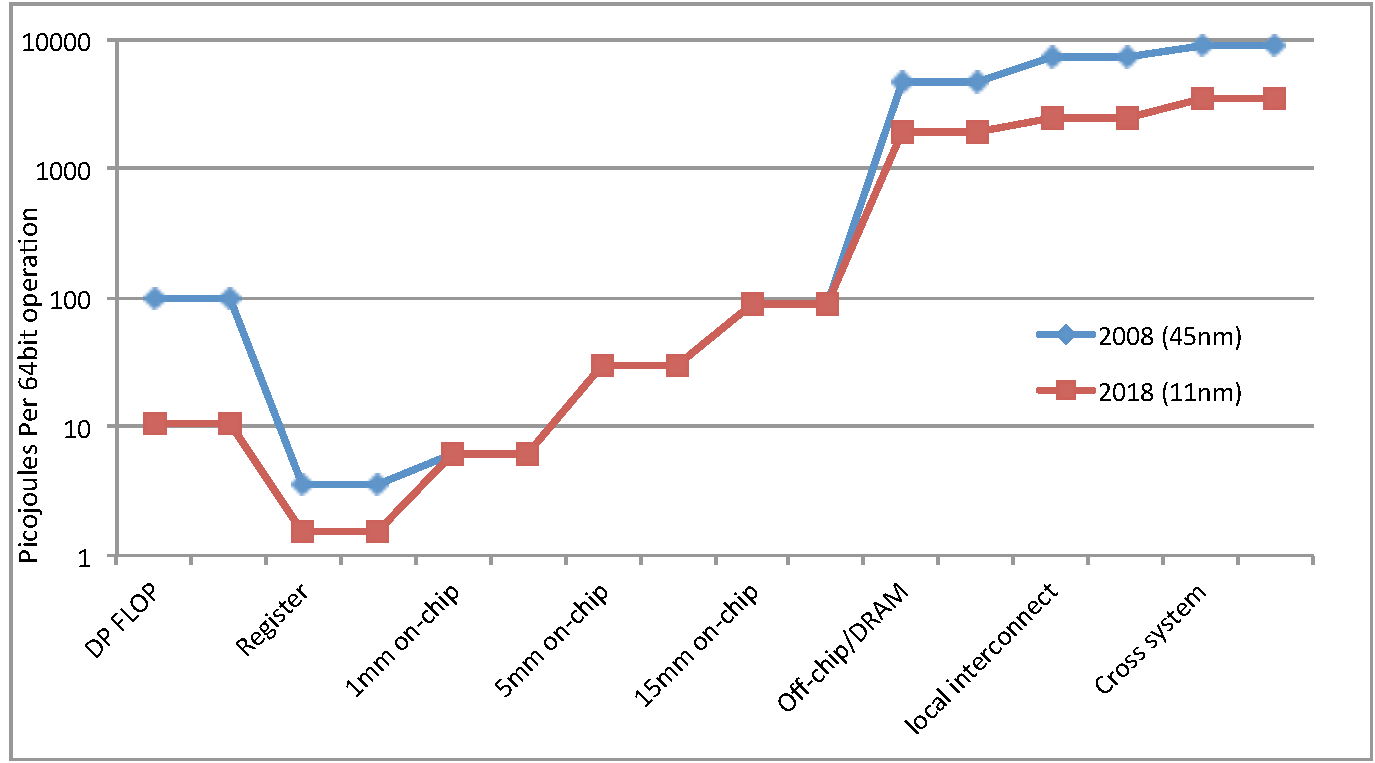
\includegraphics[width=0.95\columnwidth]{../figures/DataMovement2.pdf}
\caption{Data movement is overtaking computation as the most dominant cost of a system both in terms of dollars and in terms of energy consumption.  Consequently, we should be more explicit about reasoning about data movement. This diagram shows the cost of operations or data movement for a 64-bit operand.  By 2018, the cost of moving a 64-bit operand a mere 5mm across the chip will exceed that of a floating point operation that uses that operand. {\em The FPU and Register File energy model is computed from Tensilica's RTL design for an LX4 core with FPU.  The data movement on-chip is based on a standard resistive/capacitive model with simple signal regeneration.  The DRAM is based on Micron's projections for DDR parts.  The interconnect model is based on extrapolating historical improvements in optical transceiver efficiency and data rates.}}
\label{fig:datamovement}
\end{centering}\end{figure}

\subsection{Performance Heterogeneity}

We have evolved a parallel computing infrastructure that is optimized for bulk-synchronous execution models.  It implicitly assumes that every processing element is identical and operates at the same performance.  However, performance projections out to exascale in figure~\ref{fig:energy-per-flop} show that the only technological path that has a hope of achieving exascale by 2020 involves a heterogeneous architecture consisting of both lightweight and heavyweight cores.  Even if you are not enthusiastic about the complexity of programming heterogeneous compute engines (hybrid/accelerated computing), application developers will still need to confront heterogeneity even for homogenous processor technology.
Emerging adaptive algorithms, near-threshold voltage operation, and clock-speed throttling challenge current assumptions of uniformity.
Since the most energy-efficient FLOP is the one you do not perform, there is increased interest in using adaptive and irregular algorithms to apply computation only where it is required, and also to reduce memory requirements.  Even for systems with homogeneous computation on homogeneous cores, new fine-grained power management makes homogeneous cores look heterogeneous.  For example thermal throttling on Intel Sandybridge enables the core to opportunistically sprint to a higher clock frequency until it gets too hot, but the implementation cannot guarantee deterministic clock rate because chips heat up at different rates.  In the future, nonuniformities in process technology and Near-Threshold-Voltage (NTV) for ultra-low-power logic will create non-uniform operating characteristics for cores on a chip multiprocessor.  Fault resilience will also introduce inhomogeneity in execution rates as even hardware error correction is not instantaneous, and software-based resilience will introduce even larger performance heterogeneity.

So even homogeneous hardware will look increasingly heterogeneous in future technology generations.  Consequently, we can no longer depend on homogeneity, which presents an existential challenge to bulk-synchronous execution models.  This has renewed interest in alternative execution models that are better able to accommodate performance non-uniformity.  For example ETI Swarm, ParalleX, and Charm++ posit a completely asynchronous execution methodology that enables parallelism to be derived from concurrent scheduling of independent work rather than just by data decomposition.  These techniques that borrow much from coarse-grained dataflow methods are garnering renewed interest because of their ability to flexibly schedule work and to accommodate state migration to correct load imbalances and failures for this kind of functional partitioning model.



Performance heterogeneity offers a number of challenges to conventional approaches to data management.

1) Breaking lexical order execution of programs
2) Balancing data locality with optimal scheduling
3) Isolation of side-effects
4) Abstractions for over-decomposition


        \chapter{Motivating Applications and Their Requirements}
\label{ch:apps}



SUMMARY POINTS
Agreements

* Non negotiable : a stable program paradigm with a life cycle that is
   at least several times that of the development cycle for
   application codes
   - Applications are leery of adding dependencies
   - Code transformation to another high level language may be
      suboptimal, but maybe more attractive to apps
   - Apps are less skeptical of forms of embedded notations (DSLs or
   libraries) than full languages

* Application development often locks in data structure before fully
   fleshing out the algorithm. A formalism that imposes the discipline
   of algorithm before the data-structure might result in more
   opportunity for data locality in the app
   - In general constraining semantics is desirable as long as the
      users can override the constraints when they really need it
   - Inling assembly in performance critical sections is still
      practiced
 
* Data models are often very clear for the application, but it is not
  always possible to express them as a programming construct

* (This is not yet a general agreement, but I hope people can be
   persuaded) An application with more than one model needs a
   composable framework that can stitch together diverse data
   management demands placed upon the machines by different
   algorithms. (We agree that we need composable applications, but not
   that frameworks are the obvious choice to do that)

* Tool-chain supporting the incremental migration to the new
  programming paradigms are extremely important 
  - In order to verify the correctness in the intermediate stages of
     migration  
  - Also in general 


Disagreements

* Whether frameworks are the answer: can they handle really divergent
  sets of models in the same code
* Users appear to be voting with their feet by using python and
  matlab, should we be even concerned with new languages
  - there are limitations to using those models for HPC
  - They use low level libraries and high level constructs for
     composability, maybe that is a workable model ?

Things to Ponder
* Communication avoidance algorithms are essentially a way of
  horizontal caching (as opposed to vertical caching in memory
  hierarchy) 
* Should be able to express locality in the data structure, something
  that not only does not exist now, but also there is no theory for
  it. In fact there is no theory for data movement. (I think this
  point is extremely important)
* Should caching and redundant computations co-exist ? YES
* Would scratch-pads be better than caches (possibly)
* What is the optimum level of abstraction (translate a PDE into a
   solver, which is clearly intractable, or abstractions at the level
   of a functional module (probably still too ambitious) or something
   lower 
* The chicken-and-egg-problem of DSL/language design-is it possible to
   create something general enough that can become its own open source
   community ?



SKELETON
Motivating Applications and application requirements:

In this section we discuss data locality from the applications
perspective, covering a range of modeling methods. While the
applications space itself is very large, the set of
applications/applications experts included in the workshop do a fairly
good job of spanning the range of basic algorithmic technology in
majority of applications. They also represent the multi-physics
applications that combine several different algorithmic technologies
into one tightly coupled whole and therefore cover the biggest
challenges faced by the applications. The representative set
includes climate modeling \cite{cosmo},  molecular dynamics
\cite{gromacs}, .... , applications with structured \cite{chombo}  as well as
unstructured \cite{}  mesh refinement, particle and mesh methods, and
medical image processing. The represented problems also have varying degrees
of arithmetic intensity and potential for data locality inherent to
them. For example, Gromacs has a small working set size for (?
short-range) .... therefore good data locality. And low enough
resolution required for long range that the needed FFT's can be
confined to a small subset of processes, thereby maintaining
reasonable data locality. Whereas typical low order PDE solvers have
low arithmetic intensity and multidimensional data, which poses a
challege for exploiting data locality. Others fall somewhere in between.
Multiphysics applications face issues with data locality in another
important way because they have more than one model to solve and the  
memory access patterns are different from different models. Therefore
increasing locality for one model can result in decreasing locality
for another. 

There are well known and valid concern among the applications
communities about wise utilization of the scarcest of the resources,
the developers time, and protecting the investment already made in the
mature production codes of today. The most important consideration for
the applications community, therefore, is the time-scales of change in
paradigms in the platform architecture and major rewrites of their
codes. A stable programming paradigm with a life-cycle that is several 
times the development cycle of the code must emerge for sustainable
science. The programming paradigm itself can take any of the forms
under consideration, such as domain-specific languages, abstraction
libraries or full languages, or some combination of these. 
 
Subsection 1. The State-of-the-Art
* Those that don't have their heads in the sand are experimenting with
   techniques under consideration for exascale
   -Frank's DSL, OP2 for unstructured meshes, microblocking in AMR,
     DSLs in Cosmo, SIMD for non-bonded interations or ensemble
     simulations in Gromacs 
* Hampered in their efforts by not having a stable paradigm to program
  to 
   - Resorting to boutique solutions with varying degrees of success
   - OK for the near term, but unsustainable for the long term

Subsection 2. The Challenges
* Applications are leery of adding dependencies
   - Code transformation to another high level language may be
      suboptimal, but maybe more attractive to apps
   - Apps are less skeptical of forms of embedded notations (DSLs or
      libraries) than full languages
* Data models are often very clear for the application, but it is not
  always possible to express them as a programming construct
* Should be able to express locality in the data structure, something
  that not only does not exist now, but also there is no theory for
  it. In fact there is no theory for data movement. (I think this
  point is extremely important)
* Application development often locks in data structure before fully
   fleshing out the algorithm. A formalism that imposes the discipline
   of algorithm before the data-structure might result in more
   opportunity for data locality in the app
   - In general constraining semantics is desirable as long as the
      users can override the constraints when they really need it
   - Inling assembly in performance critical sections is still
      practiced
* The chicken-and-egg-problem of DSL/language design-is it possible to
   create something general enough that can become its own open source
   community ?

Subsection 3. The Wish List
* Non negotiable : a stable program paradigm with a life cycle that is
   at least several times that of the development cycle for
   application codes
* Should be able to express locality in the data structure, something
  that not only does not exist now, but also there is no theory for
  it. In fact there is no theory for data movement. (I think this
  point is extremely important)
* Tool-chain supporting the incremental migration to the new
  programming paradigms are extremely important 
  - In order to verify the correctness in the intermediate stages of
     migration  
  - Also in general 


Subsection 4. Research Areas
* What should a multi-component application framework look like in
   order to maximize data locality in view of diverse and conflicting
   demands of data access patterns. 
* If formalism existed for defining data movement, how can the apps
   be configured to exploit it
* Would scratch-pads be better than caches, or should catching be
   both vertical and horizontal
* What is the optimum level of abstraction (translate a PDE into a
   solver, which is clearly intractable, or abstractions at the level
   of a functional module (probably still too ambitious) or something
   lower 

       % !TEX root = ../padalreport.tex
\chapter{Data Structures and Layout Abstractions}
\label{ch:datastructures}


%Define your Area
%  Create definition of your research area
%  Describe key concepts that define your area or that were uncovered during the course of conversation
%  A few examples of work in that area (can refer back to talks on website, but no need to recount entire talk)

%Findings:
%■ Describe points/observations/discoveries/challenges/issues uncovered in the session
 %● Distill into summary (major discoveries)
 %● can refer back to presentations for details
 %● Can also use data from panel discussions
%■ Identify areas of agreement
 %● Common approaches
 %● Common concerns
%■ Identify areas of disagreement
 %● what is the substantive cause of the disagreement (document)
 %● What metrics/information/research are needed to compare/resolve
%■ Identify Gaps
 %● What is missing?

%Recommendations
%■ Opportunities for standardization of mature technologies where the is substantial agreement or commonality
 %● Have we met the necessary conditions for standardization (is the area well enough understood, are the elements of existing implementations sufficiently similar, are the benefits clearly demonstrated, is there a user community?)
 %● What should we standardize? ( Low­hanging fruit )
 %● How can we influence standards committees? (e.g. C++17standards committee?)
%■ Define research agenda for new ideas or areas where there is insufficient information to choose a final implementation ( What areas need more research?)
 %● identify research thrust
 %● what are the opportunities
 %● what needs to be done
 %● What needs to be prioritized?
 %● What resources would be required (estimate size/complexity ofthe problem if you can)
%■ How do we create a user community? (bonus question)

\section{Introduction}
\note{Scroll down to see the original outline}


Lack of a single abstract machine model  due to the diversity of the architectures 
requires the programmer to support various implementations of the same program to achieve high performance
on different platforms. Recently, a number of programming interfaces such as Kokkos, TiDA, OpenMP
extensions, GridTools, Dash, Array Extensions \cite{all} have arise to give developers more control over 
 data layout and to abstract the data layout itself from the application. 
 In this chapter, we discuss the key points when designing such abstractions, emerging approaches with (im)mature
 solutions, and potential research areas. Here, we focus on  locality management on data-parallel algorithms 
 and leave the discussion on task-oriented abstractions to Chapter~\ref{ch:taskmodels}.

Before going into further discussions, let us define relevant terminology. \note{I sent an email 
for discussion, will update this section based on the responses.}
We consider {\em data structure} as an organized collection of 
datum residing in one or more memory spaces (e.g. main memory, local storage).
{\em Data decomposition} is partitioning of data collection into smaller chunks with the intent of fitting small chunks into certain memory space or introducing more parallelism. 
{\em Data placement} maps each partition of data collection onto memory spaces. 
{\em Data access pattern} is the access order to the data by the computation's algorithm and its execution policy and might be different than storage pattern.
{\em Execution policy (Thread Binding?)} determines how tasks are scheduled and mapped onto data collections. 
{\em Data layout} refers to the policy that decomposes data, uses a certain storage pattern and determines placement of data onto memory spaces, 
typically with the intent of efficient and performant access by a collection of computation.  

\note{There is also data distribution. I am not sure how this is different than data placement. }
  
  
\section{Key Points}
It is encouraging that there is a shift towards a more data-centric programming in the research community. 
We consider the following design principles as important and desired by the application programmers.

\begin{itemize}
\item Separation of concerns is important to maximize expressivity and optimize performance. That principle is applied to the distinction between a logical, semantic specification, and lower-level controls over the physical implementation.
 At the semantic level, scalar work is mapped onto parallel data collections, using logical abstractions of data layout which best promote productivity. Domain experts can also expose semantic characteristics like reference patterns that can inform trade-offs made by tools.
\item Performance tuners, who may be distinct from the domain experts, may exercise control over performance with a set of interfaces which can be distinct from those that specify semantics. 
\item Through these interfaces, they may decompose, distribute and map parallel data collections onto efficient physical layouts with specialized characteristics,
\end{itemize}

\note{Move the following to discussion?}
The key point of separation of concerns is of offering, to the user of
the interface, an architecture agnostic {\em abstract machine}
(AM). An AM is necessary to express an algorithm, being it a
functional language or a Turing machine. An algorithm written for an
AM must be translated into program for a {\em physical machine} (PM),
which can be closely related to AM or completely different. The
translation effort depends on the ``distance'' between the AM and the
PM. Since there are many different PMs, and the lifetime of
applications should be much longer that the lifetime of an
architecture, the usual request is that an algorithm for an AM should
be executed efficiently in the widest possible class of forseeable
PMs. This is the well know problem of {\em portable efficiency}. From
this perspective an AM should be distant from PMs for two reasons:
first it gives the user an uniform view of the porgramming space,
often at a much higher level of abstraction than any specific
programming model for a PM; second, the hope is that by being
equidistant from any PM the translation can lead to equally efficient
implementations with similar effort.

The interfaces the Authors of this report are developing, the already
cited Kokkos, TiDA, OpenMP extensions, GridTools, Dash, Array
Extensions, provide AMs at widely different abstraction levels. Some
as DASH provide a PGAS abstraction in C++, so that DASH AM is
basically an universal parallel machine with the concept of (two
levels: local and remote) locality made explicit. GridTools provides a
set of libraries for expressing distributed memory implementations of
regular grid applications, like stencils. It is not meant to be
universal, in the sense that non regular grid applications should not
be expressed using Gridtools libraries, even though possible in
principle, for performance reasons. Since the constructs provided by
GridTools are high level and semi-functional, locality issues are
taken into account at the level of performance tuners and not by
application programmers. At user level the locality is take into
consideration onlyh implicitly. Kokkos is a library for expressing
multidimensional arrays in C++, in which the layout can be decided at
compile time. An algorithm written with Kokkos uses the AM of C++ with
the data specification and access provided by the interface of Kokkos
arrays. Locality is managed explicitly by matching the data layout
with the algorithm logical locality. \note{Not sure what to say about
  the others}. As can be seen, there is not a single way of treating
locality concerns, and there is not consensus on which one is the
best. Each of these approaces are appealing to different scenarios
that depends on the scope of the particular projects. In the case of
C++ libraries, anyway, there is the possibility of naturally building
higher level interfaces using lower level ones, for instance a DASH
multidimensional array could be implemented using Kokkos arrays, and
GridTools parallel algoritmhs could use DASH library, and Kokkos
arrays for storage, etc. This is a potential benefit from
interoprability that arises from using a commom language provided with
generic programming capabilities, as C++.

\note{The followings were used to be in the terminology but I think we
  center the discussion around them. Mauro: I think they should be
  moved to the terminology section.}

\begin{itemize}
 \item Memory access pattern: The memory access pattern of a computation is determined by the composition of the computation's algorithm, computation's execution policy, and layout of the computation's data structures.  The quality of a computation's memory access pattern is determined by the time or energy consumed accessing its datum.  

  \item Polymorphic layout: The quality of a computation's memory access pattern may depend upon the architecture of the computer on which it executes.  A data structure has a polymorphic layout if the layout can be changed to improve the memory access pattern without modifying the source code of computations depending upon that data structure.

  \item A data structure (-layout) has good locality (-behavior) with respect to an algorithm if operations on the data structure can be executed efficiently in terms of run-time and/or energy consumption. So locality is not a property of the data structure or layout alone, there is an execution/code component that determines if locality behavior is good.

  \item Algorithmic locality vs. actual/implementation locality: An algorithm is expressed in terms of operations on certain abstract data types, such as matrices, trees, etc. The algorithm code usually express access patterns to the data at high level, such as accessing the parent node in a tree, or the elements in a row of a matrix. This express a {\em logical locality}, that we refer to {\em algorithmic locality}, since it may be not related to the {\em actual} or {\em implementation} locality, that express the locality characteristics of locality of the code obtained by mapping the algorithm (maybe through a compiler) to the physical architecture. \note{Mauro: tried to clarify this. Does it work?}
 \end{itemize}

\section{Emerging Approaches}
Here we may want to discuss Kokkos, TiDA, GridTools etc a little bit (few sentences for each)

\section{Discussions or Challenges ?}

Libraries? 
Flavors of functional programming ?

The choice of base language to implement the mentioned abstractions varies among different groups. 
Some prefer standard languages such as Fortran, C/C++ in order to maximize impact and leverage market breadth of the supporting tool chain (e.g., compilers, debuggers, profilers). Wherever profitable, there can be a push to �redeem� existing languages by amending or extending them, e.g. via changes to the specifications or by introducing new ABIs. It is noteworthy that the ISO C++ standardization committee intends to address performant, on-node parallelism in a future language standard.
C++ meta-programming can cover a significant fraction of the desired capabilities, and that it�s a middle road for being able to implement DSLs that are embedded within standard languages. Specialization can be hidden in template implementation and controlled by template parameters. Even though there are a huge number of applications implemented in Fortran, 
there is a concern about Fortran's lack of extensibility in terms of lambdas and templates. Others believe that specialized languages are required, e.g. to �get us to exascale.� Different language rules may be required to overcome limitations imposed by current languages. For example, C exposes physical data layout, and limits a compiler�s ability to re-layout data. Source to source translators are still subject to language rules, whereas new languages may remove such limitations through abstraction.
In conclusion, there is no single language  to physically implement the layout abstractions 


\section{Research Areas}



\section{OUTLINE}

HIGHLIGHTS

\begin{itemize}
\item SCOPE
  \begin{itemize}
  \item In this chapter, we discuss language and library interfaces that help manage programming abstractions for data locality, particularly for data structures and data layout. 
  \end{itemize}
\item KEY POINTS
  \begin{itemize}
  \item \note{Didem: I think this should appear in the introduction of the entire report.}What are the {\em easy} and the {\em complex} parts of algorithm design? I think the {\em easy} should include parallelism. From the implementation point of view this may be different, but compared with the challenges of locality, parallelism should be considered easy and high level. What is the level of ``algorithmic locality'' that we want to be able to specify? Is local/non-local distinction sufficient?
  \item From the requirements of the applications (and scalability) we focus on data-parallel algorithms (even though we may use task oriented abstractions and runtimes).
  \item The lack of a single abstract machine (programming model) to program for performance imposes the choice of data-structure specific constructs and specific implementations of those for different platforms (for now this is an empirical observation)
  \item \note{not sure I got this item, it seems similar to the item right above}The diversity of the architectures also forces these constructs to work at level of {\em means of combination/composition} (it's not sufficient to provide very efficient primitive operations, like BLAS).
  \item Separation of concerns is important to maximize expressivity and optimize performance.  That principle is applied to the distinction between a logical, semantic specification, and lower-level controls over the physical implementation.
  \item At the semantic level, scalar work is mapped onto parallel data collections, using logical abstractions of data layout which best promote productivity.  Domain experts can also expose semantic characteristics like reference patterns that can inform trade-offs made by tools.
  \item Performance tuners, who may be distinct from the domain experts, may exercise control over performance with a set of interfaces which can be distinct from those that specify semantics.  Through these interfaces, they may 
    \begin{itemize}
    \item decompose, distribute and map parallel data collections onto efficient physical layouts with specialized characteristics, 
    \item map parallel work onto underlying hardware mechanisms for supporting parallelism, and 
    \item exercise control over temporal sequencing of work and movement of data for locality.
    \end{itemize}
  \item Some (im)mature solutions implemented in different languages include: Kokkos, TiDA, OpenMP extensions, GridTools, Dash, Array Extensions
\end{itemize}


\item TERMINOLOGY (define each of these up front)
  \begin{itemize}

 \item Data structure: A organized collection of datum residing in one or more memory spaces. 

  \item Layout (of data structure):
    The mapping of a data structure into one or more memory spaces, typically with the intent of efficient and performant access by a collection of computations.

    Example: A 2D matrix of size 100x100 holding integers is a data structure: a semantic/logical entity in which a programmer thinks. Storing and processing the matrix in a computer requires a layout that maps the 2D matrix onto the 1D address space of the computer in some way. The mapping could be a simple linearization or it could be a more complex blocked (tiled) scheme.

  \item Memory space: A computer has multiple memory resources.  A single computer traditionally has main memory, one or more levels of hardware managed cache memory, and registers; where the main memory is the only memory space explicitly managed by a program.  Advanced architectures have heterogeneous memory for performance that must be managed by computations.  Examples of these memory spaces include CPUs' non-uniform memory access (NUMA) regions, separate GPU memory, and software-managed on-chip memory.

 
  \item Distributed data structure / parallel data structure: not sure we should use either of those terms, but if we do we should make sure what we mean: is the data distributed over multiple nodes/address spaces? is there concurrent access to the same data structure? 
      
  \item \note{Didem: should be part of the report intro} Locality: A measure of distance between datum on a computer.  For example, do the datum reside in the same compute node of a cluster, in the same memory space, in the same cache line?  [I can't think of a direct definition that doesn't require a whole lot of other definitions up front, so how about the following phenomenological definition?]

  \item Execution policy: How a computation's units of work are scheduled and mapped onto data collections. \note{is this the same thing as thread binding?}

  \item Memory access pattern: A computation accesses data structures according to its execution policy. 

  \item Memory access pattern: The memory access pattern of a computation is determined by the composition of the computation's algorithm, computation's execution policy, and layout of the computation's data structures.  The quality of a computation's memory access pattern is determined by the time or energy consumed accessing its datum.  

  \item Polymorphic layout: The quality of a computation's memory access pattern may depend upon the architecture of the computer on which it executes.  A data structure has a polymorphic layout if the layout can be changed to improve the memory access pattern without modifying the source code of computations depending upon that data structure.

  \item A data structure (-layout) has good locality (-behavior) with respect to an algorithm if operations on the data structure can be executed efficiently in terms of run-time and/or energy consumption. So locality is not a property of the data structure or layout alone, there is an execution/code component that determines if locality behavior is good.

  \item Algorithmic locality vs. actual/implementation locality: Not sure I would know how to define these terms. What is algorithmic locality of matrix multiplication? 

  \item Logical, semantic level: programmer expresses the WHAT, exposes OPPORTUNITY in a natural expression; portable
  \item Portable efficiency
  \item Algorithmic locality vs. actual locality or implementation locality
  \item Physical, performance level: CONTROL over HOW, so as to meet performance goals; may be implementation specific
  \item Polymorphic: may take different forms, depending on the abstraction layer or optimization target
  \item Language interface: a spec or API used by a programmer, which may be part of the base language, a compiler-interpreted directive, or a library API [this may need work] 
  \item Language construct: something that can be identified as a {\em keyword} in a language interface and the grammar rules that applies to it.

  \item Binding: mapping from the logical to physical domain, e.g. for storage
  \item {\em What follows should be either filled in or dropped}
  \item control space(use execution space?)
  \item binding  (or execution policy ?)
  \item data layout
  \item data decomposition 
  \item data distribution 
  \item iteration space traversal (avoid using loop traversal, maybe use domain traversal?) maybe : {\em iteration patterns} to be paired with {\em access patterns}?
  \item access type
  \end{itemize}


\item AGREEMENTS
  \begin{itemize}
  \item Abstractions for performance portability are needed: Data layout, tile sizes, memory access patterns need to be tuned when application is moved between machines. [We may want to tweak that list.]
  \item The separation of logical from physical concerns enables:
    \begin{itemize}
    \item Separation of concerns between domain experts and performance tuning experts
    \item Maximal exposure of opportunity, vs. hard coding a particular trade-off
    \item Getting free of enslavement to restrictions or suboptimalities imposed at the logical level
    \item Minimizing, or at least localizing, code modification for control over performance
    \item Polymorphism across targets and abstraction layers
    \end{itemize}
  \item We need a data model to assess the data locality
    \begin{itemize}
    \item We have a model for parallelism but do not have a model for data locality
    \item Optimal trade-offs may shift over time and across target systems.  
    \item Models need to take into account the capabilities and capacities of computational elements, memory structures, and the network fabric 
    \item Models should reflect the consequences of various controls, such as the placement of work near data
    \end{itemize}
  \item It's easier to standardize high-level concepts, suggesting that
    \begin{itemize}
    \item Extensions for controls over how parallel work and data are managed may best be targeted at libraries and language interfaces, rather than base languages.  There's greater freedom for diversity there.
    \item Base languages are a good longer-term target for semantically exposing opportuniteis for parallelism (and locality?)
    \end{itemize}
  \item Low hanging fruit: 
    (1) multidimensional array support (in C and C++) 
    (2) runtime polymorphic data layout: 
    ideally change the layout in runtime (it should always be clear when an operation has performance costs),
    (3) compile time polymorphic layout: change the layout at compile time with minimal code modifications, 
    support layout in the type system 
  \item Performance-related controls pertain to data and to execution policy.  These may vary in their scope and granularity.
    \begin{itemize}
    \item Data controls may be used to manage:
      \begin{itemize} 
      \item Decomposition, which tends to be either trivial (parameterizable and automatic) or not (explicit)
      \item Binding to storage: to a particular type of memory (e.g. read only, streaming), to a phase-dependent depth in the memory hierarchy (prefetching, marking non-temporal), or to memory structures which support different kinds of sharing (SW managed, cached)
      \item Mechanisms for, and timing of, distribution to data space/locality bindings
      \item Data layout
      \end{itemize}
    \item Execution policy controls may be used to manage
      \begin{itemize} 
      \item Decomposition of work, e.g. iterations, hierarchical tasks
      \item Ordering of work, e.g. recursive subdivision, work stealing
      \item Association of work with data, e.g. moving work to data, binding to hierarchical domains like a node, thread or a SIMD lane
      \end{itemize}
    \item These controls may be applied at different scopes and granularities through a varity of mechanisms
      \begin{itemize} 
      \item Data types - global, fine-grained, can vary by call site
      \item Function or construct modifiers - local coarse-grained, can vary within a scope
      \item Environmental variable controls - global policies
      \end{itemize}
    \end{itemize}
  \item lambdas for domain traversal (or iteration space traversal) [is this now adequately covered below?]
  \end{itemize}
  
\item  DISAGREEMENTS
  \begin{itemize}
  \item Binding [could someone flesh out the opposing points of view?] Depending on the level at which a language/library stands (single thread, multicore chip, parallel distributed system) the binding is responsibility of the user or the system. I don't think we agree on what the level of abstraction is right, so we could not agree in the binding, I guess.
  \item support for memory spaces: can be hidden from the programmer or exposed [could someone flesh out the opposing points of view?]  Traditional architectures have hidden memory spaces within node through hardware supported movement of datum through a cache memory hierarchy.  This implicit memory space management strategy has been applied to distributed memory clusters through PGAS programming models and runtimes.  There has is not a consensus on PGAS versus explicit management of datum movement among clusters' compute nodes.  Advanced compute node architectures have heterogeneous memory spaces which must be managed for computational performance.  It is an open question as to whether a programming model can be deployed that implicitly manages these memory spaces and provides sufficient memory access quality.

  \item Choice of language interfaces
    \begin{itemize}
    \item Some prefer standard languages, in order to maximize impact and leverage market breadth of the supporting tool chain (e.g., compilers, debuggers, profilers).  Wherever profitable, there can be a push to ``redeem'' existing languages by amending or extending them, e.g. via changes to the spec or by introducing new ABIs.  It is noteworthy that the ISO C++ standardization committee intends to address performant, on-node parallelism in a future language standard.
    \item Others believe that specialized languages are required, e.g. to ``get us to exascale.''  Different language rules may be required to overcome limitations imposed by current languages.  For example, C exposes physical data layout, and limits a compiler's ability to re-layout data.  Source to source translators are still subject to language rules, whereas new languages may remove such limitations through abstraction.
    \item There's some agreement that C++ metaprogramming can cover a significant fraction of the desired capabilities, and that it's a middle road for being able to implement DSLs that are embedded within standard languages.  Specialization can be hidden in template implementation and controlled by template parameters.
    \item There's some concern about Fortran's lack of extensibility, e.g. in the direction of lambdas, templates and metaprogramming
    \end{itemize}
  \end{itemize}

\item GAPS (what is missing? not covered at the workshop)
  \begin{itemize}
  \item A data model for which data layout is more suitable for which algorithm? or metric for locality
  \item The mentioned distinction between WHAT and HOW is subtle. I think every developer is concerned with WHAT. As library/language developers we want our users to be concerned by certain WHAT that we turn into HOW by stating some lower level WHATs. In my work I can use a PGAS approach (in which locality is expressed as a here-or-there) underneath but hide it altogether to my user. I think we disagree at what level our users should express their programs. We agree that there must be a separation of concerns but not where the separation should be.
  \end{itemize}

\item RESEARCH AGENDA
  \begin{itemize}
\item If we speak of data locality, is a binary local/remote distinction enough or do we need a more fine-grained differentiation? If so, what is the best way to represent and measure this multi-level locality concept. Is "hierarchy" always the right concept and is a tree always a good representation?

\item What about horizontal locality management vs. vertical locality management? Do they require different abstractions or can they be handled in a uniform way?

  \item Identify minimal set of data and execution policy controls
  \item Compare/contrast available options for specifying those controls
  \item Identify gaps and prescribe steps toward closure of those gaps
  \item Converge on a minimally set of (semi-standard) solutions that provide adequate coverage
  \item Prove or disprove that an portable efficiency can be achieved with a single language (in order to prove or disprove that data-structure specific approaches are the only beign possible)
  \end{itemize}

\end{itemize}




       \chapter{Language and Compiler Support for Data Locality}
\label{ch:langcomp}

%%% STRUCTURE:
%%% At the start, in comment - Notes from the google doc we discussed at the meeting
%%% At the end, in comment - Notes from the two scribes
%%% Outline - modelled on what the datastructures group did

%% NOTES FROM THE GOOGLE DOC WE DISCUSSED AT THE MEETING

%Define your area
% - create definiition
%	To maximise portability we need the user-facing level to be … while 
%	Differentiate languages/compilers/tools from models, libraries, active libraries, embedded DSLs
%	Polyhedral?
%	Identify and recognise that solutions operate at different levels of abstraction and automation (“multiresolution”)
%	Principle: avoid losing information, premature lowering
%	Principle: isolate cross-cutting locality concerns
%	cf rank-independence
% - key examples of work in the area
%	HPF (and Brad’s blog) - vagueness - robust, well-defined, well-understand abstractions 
%	UPC (need to have clear ambitions/capability beyond the low-hanging fruit)
%	Research vehicles can be narrow but a basis for a standard has to have potential for beyond
%	Titanium, Global arrays
%Conflict between local-view vs global view (clarify the difference - 
%* Findings
% - agreement	
%There’s a lot of consensus around multidimensional data/partitioning/slicing, and how to iterate over them (generators, iterators) - parameterisation of layouts.
%There’s potential to expose polyhedral concepts to the programmer/IR, and to pass them down to the backend (eg Chapel’s domains, mappings)
%The back-end model for the target for code geenration and implementation of models/compilers is “missing” - for portable implementation, for interoperability
%While we can do a lot with libraries and template metaprogramming, there is a compelling case for a language-based approach
% - differences
%No consensus on the requirements on intermediate representations and runtime systems
%Do what I say vs do what I mean
%Compositional metadata vs explicit dependence/synchronisation/movement (Brad has words)
%	
%
%* Recommendations:
%  - Opportunities for standardisation of mature technologies
%  - What is this standardisable low-hanging fruit?
%  - how to influence standards?
%  - define research agenda
%Scope out the opportunities for JIT - plenty of compelling need for infrastructure (specialisation, autotuning, …) [[what’s the research agenda/challenge here?]]
%  - how do we create a user community?
%
%* Seek input from key participants, esp speakers from our session
%
%Two-page exec summary, 30 page total.  So we’re talking about 3-5 pages.





%%%% NOTES FROM THE SCRIBES
%
%Anshu:
%
%Q. Why a language rather than library, and paths to make it easier 
%to make your language/library adopted
%
%- They are not mutually exclusive, despite long odds we need to keep striving
%   for languages. 
%- Practical reason - syntax matters, things like inferred type and optimization 
%   opportunities better expressed
%- The biggest challenge is getting adopted
%- Academic languages have more challenge to adoption 
%- Template meta programming covers a good percetage of what a language provides
%- The two DSLs based on Python etc they are libraries developed at first by
%    the domain people 
%- Strategically led by applications, essential to maintain the engagement.
%- In order to engage with users - one has to compete with 
%   everything else available
%- Common backend -- target backend c compiler and then provide
%   an appropriate design, take it down to more explicit form 
%- Source to source translator is preferable also for greater portability
%
%- Adoption problem - there is a real hunger for a new language so no excuse for
%   not developing one
%- CUDA- adoption - more than a million downloads, even with small changes
%    timing is important, the real complaint is it only runs on nvidia 
%- Complete rewrite is a red-herring
%
%- The whole tool chain is important,  and interoperability is the key 
%
%Q. What is missing from a common backend 
%
%- targetting C- as a good portable assemble language 
%- 1D array limitation, there is a movement for 
%    support of multi-dimension arrays in C++
%- parallelization/vectorization information
%- lack of any locality information C or C++ how to address it
%- locality is useful even for exploiting memory hierarchy
%- C++ standards committee- all volunteer -- you join ISO pay the fee
%   and then you join the committee and then you attend a few meeting
%   to earn the voting rights
%
%- Locality info is not just hierarchy or also adjacency (helpful for stencils)
%- polyhedral - could be the intermediate information - but the info
%- from the source is lost. How to get this information from the source
%
%- synergy between iteration spaces and domains in chapel, could that
%   be exploited ?
%- X10 is doing polyhedral optimizations, XL compilers are also using it
%   if there is a possibility of closer cooperation
%
%- Polyhedral - parameterization of linearization, the problems that 
%   are coming out are really really hard. You need an affine, most
%   machines cannot be modeled, so then you need hacks. It is
%  a nice mathematical model but not the panacea. 
%- Limitations - Associavity 
%
%- discussion goes back to imperative Vs declarative 
%   with polyhedral model - extracting the representation 
%   from the source code, or you can write into a DSL and emit
%  the source. Once you have lifted away from having to extract
%  the model why constrain ?
%
%- This is because the community knows how to solve the convex
%   optimization problems but not much as. 
%- The other side is correctness, the limiting factor. 
%
%- Calculus of problem transformation, separate from the actual
%  optimization. Which transformation to apply to what optimization
%  not too many are optimizations are applied all at once.
%- Restrictions imposed by the 
%  polyhedral model, interesting cases is when the subscript case
%  is indirection - is the meta-data becomes bigger than the data
%  so it has to done at runtime
%
%- Automatic compiler techniques - have them for years auto-parallelization
%   we gave up on it, so are we going back to it.
%
%- Data locality -- instead of expressing where the data is, but express
%   implicitly the relation and hierarchy, sufficiently broad possibilities
%   so that it can support a range of back-ends. 
%- In stencil explicitly specify the shape of the stencil, sometimes 
%   you can generate automatic parallelization
%- Right container libraries or constructs will be helpful
%
%- Robustness--if you are counting on the compiler to do auto-parallelization
% for you it needs to be robust. 
%- Data movement implied by the parallelism,
%  what the data access footprint of the loop is. If you break that, the compiler
%  should be able to tell you. Column major Vs row major, if there is a transpose
%  the profiler should point out. Anamoly detection.
%- Expressing locality should be portable, pushing that from applications space
%   to the runtime space. May be unrealistic to push it to the compiler space.
%- Whether all the things should be visible in the syntax of the data structure
%  nice for analysis, the flip side is lack of portability. Ability to reason about
%  the locality in semantic ways is more important, ability to put in assertions
%   and then tools. 
%- Locality and profiler -- how much can a compiler do
%
%- whether your code expresses its belief about its performance characteristics
%- semantic information conveyed to the system could be statically
%   analyzed, the compiler may make the decision to utilize it.
%- The ability to express in a language may be exploited first at the runtime,
%   rather than the compiler.
%- Compositionality - communication and the locality depends on the context.
%
%
%Didem:
%
%Language and Compiler Support for Data Locality 
%
%Why a language rather than a library?
%Brad: fully adapted, pursing lanauge. Keep trieving a lanaugeg because 
%in the long term people want lanauge, syntax matters a lot 
%hard to do in a library, optimization opportunies for compiler 
%
%Amir: Titanium, no one used it. Things are different when vendor supports. 
%Users think that the language 
%Language provides many opportunies 
%Embedded DSL and metaprogramming is a good alternative. 
%We can get most of the lanauge provides. 
%
%Paul: both his DSL are libraries. not language 
%strategically he has to engage with app ppl. It is important to work the app ppl. 
%I am agnostic about how it is deliver to you(compiler). How you get it 
%it is not important. Delay execution
%
%Armind: barrier to adopting a new language is hard 
%syntax extensions are possible 
%
%Cj: go after users? if you want to be portable
%John: if you don't have a common back 
%
%Amir: src-to-src translators address that
%
%Naoya: compiler doesn't mean all the way from high to asembly 
%but to some intermediate form 
%final output is left to the vendor compiler 
%
%Brad: there is a true hunger in users. Users do not have a choice 
%because it is hard because it is no user group, we shouldn't develop a new langa
%that's wrong , that's a dissoppioiting excuse.
%
%Peter: about CUDA, we have 1M downloads. Few syntactic changes, and people 
%are complaining. wondering about timing 
%
%Brad: why java and python are new language and they got adopted. 
%great interoperability 
%
%Didem: complaint about CUDA is not the extension but optimizations 
%because it requires a lot of rewrite of the code 
%
%Carter: entire tool chain change required for CUDA
%
%Anshu: interoperatability is important for a new language because 
%you have to rewrite entire your code 
%
%Brad: he agress interoperatbility. 
%
%John: DSL and lang targetting LLVM  
%is the question what is missing in common backend to inhibits your locality optimizations?
%what is missing in LLVM? or IR?
%
%Brad: targetting C, it is portable assembly 
%multidimensional arrays are missing. C++ next standard is targetting multidim 
%arrays, that will be great. 
%
%Amir: targetting C and C++, lack of any locality information are missing 
%C++11 has some model for parallelism. 
%
%Didem: How to influence C++ committee to address HPC needs?
%
%Carter: join ISO first. pay C++17 ISO join fee
%certain number of meetings to earn voting 
%
%....
%
%...
%
%Armid: annotation and better langauge can provide more info to polyhedral
%LLVM is too low level close to assembly with type info 
%
%...
%
%Kathy: IBM is now working with polyhedral and it is actually XL compiler 
%
%John: algebraic model, data model theory?
%
%Torsten: only applicable to DSL, to fine domain. 
%parameterized integer programming is not pragtical.
%it not a panacea
%
%Thomas: users need something different than imperative langauge 
%python 
%pollyhedral models fall back into 
%
%Torsten: you can extract the poly representation from the source, that source can be 
%anything. convex optimizations, affine functions are easier to solve in the compiler. 
%So it is good that ployhedral constrains your source 
%
%Armind: preserve the correctness of the program, that's the limiting factor 
%the user shouldn't see what's going on 
%
%Padua: optimization process is different that poly 
%
%Armind: objective function 
%we apply opitmizations in order, first parallelization, then locality and then tiling etc. 
%
%...
%
%Paul: people are talking about restrictions of ploy. that's actually great 
%indirection is interesting, metadata that charactizing the iteration space 
%that has to be done in runtime 
%
%
%John: How do we make the data locality and data movement in a program robustly evident in the code?
%what additional information do you need from programmer (model)?
%We gave up on auto parallelization and auto data locality.
%
%Peter: explicitly declared the proximity of the data in Pylaxn
%
%Naoya: in a stencil case, explicitly define stencil shape. COmpiler can generate optimized code.
%even for distributed memory. 
%
%Armind: right data structure 
%
%Paul: 
%1) robustness: in a good day, it gives good performance but always but you need robustness. 
%When the user breaks he knows. 
%
%2) Data movement: how data is distributed
%data access footprint 
%sometimes you need to even declare it 
%
%3) loop 1 and loop 2 : between the two, all to all broadcast. 
%suddenly, it
%profiler should tell you about this bottleneck
%
%Amir: data locality in a portable manner 
%Peter had the right idea. push it from the application to runtime. 
%Pushing to the compiler is too hard. Runtime can do better job. 
%
%Brad: Making the movement explicit 
%it doesn't need to be syntactically 
%all the communication is exploict in the langauge. 
%It had a drawback. because it is portable
%Syntaxtically in Chapel we avoided that. 
%Semantically expressing data locatity is the way to go not syntaxtically 
%
%Padua: how much can compiler do? 
%it is temporaily in the language until the compiler 
%
%Paul: performance properties of your code. If I break your assumptions, 
%I want to 
%compiler fails without an explanation. 
%
%Satoshi: semantic info can convey should be something should 
%be dynamic, hand to the runtime. Some of them can be statically analzyed in the compiler. 
%
%JOhn: HPF had the mistake that putting everything to the compiler. 
%
%Paul: composition: locality depends on the context 

\section{Introduction}

{\it
SCOPE
  \begin{itemize}
  \item In this chapter, we discuss language concepts for data locality, their delivery in general-purpose languages, domain-specific languages and active libraries, and the compiler technology to support them.
  \item We explore the proposition that management of locality in parallel programming is a \emph{language} problem.
  \item Language-based solutions may come in the form of new, general-purpose parallel programming languages.  As well as supporting intuitive syntax, doing so creates the scope for ambitious compilation techniques, sophisticated use of type systems, and compile-time checking of important program properties.  
  \item Language concepts for locality can also be delivered within existing languages, supported in libraries, through metaprogramming in C++, and in ``active libraries" with library-specific analysis and optimizations.
  \item Locality is about data, and locality abstractions refer to abstract data types.  Multidimensional arrays are a crucial starting point.  Many more complex domains can be characterized by the abstract, distributed data structure on which parallel computation occurs.  Domain-specific tools are often focussed on particular data structures - graphs, meshes, octrees, structured adaptive-mesh multigrids etc.  While Chapter~\ref{ch:datastructures} tackles particular data structures, in this chapter we look at how to build tools to support programmers who build such abstractions.
  \end{itemize}
}

Locality is a fundamental concern for current and future HPC architectures, since the cost of data movement defines a large fraction of overall application performance. The concept of locality, however, has not yet become a first-class citizen in general-purpose programming languages. As a result, although application programmers are often confronted with the necessity of restructuring program codes to better exploit locality inherent in their algorithms, even a simple simulation code can become highly non-intuitive, difficult to maintain, and non portable across diverse architectures. 

The overarching vision of this workshop is to solve these issues by presenting application programmers with proper abstractions for expressing locality. In this chapter, we explore the proposition that management of locality in parallel programming is a \emph{language} problem. More specifically, we discuss language concepts for data locality, their delivery in general-purpose languages, domain-specific languages and active libraries, and the compiler technology to support them. 
 
Language-based solutions may come in the form of new, general-purpose parallel
programming languages.  In addition to supporting intuitive syntax, language-based approaches enable ambitious compilation techniques, sophisticated use of type systems, and compile-time checking of important program properties. Language concepts for locality can also be delivered within existing languages, supported in libraries, through metaprogramming in C++, and in ``active libraries'' with library-specific analysis and optimizations.
 

Locality is about data, and locality abstractions often refer to abstract data types. Multidimensional arrays are a crucial starting point.  Many more complex domains can be characterized by the abstract, distributed data structures on which parallel computation occurs. Domain-specific tools are often focused on particular data structures---graphs, meshes, octrees, structured adaptive-mesh multigrids, etc.  While Chapter~\ref{ch:datastructures} tackles particular data structures, in this chapter we look at how to build tools to support programmers who build such abstractions.

Locality is also about affinity---the placement of computations (e.g.,
tasks) relative to the data they access.  Dominant HPC programming
models have typically been based on long-running tasks executing in
fixed locations fetching remote data.  Emerging architectures may also
compel us to pursue languages in which computations are moved to the
data they wish to access.  To implement such models, languages will
need to also support the creation of remote tasks or activities.

The following terms are used in this chapter:

\begin{itemize}
\item \emph{Active library:} a library which comes with a mechanism for delivering library-specific optimizations~\cite{DBLP:journals/corr/math-NA-9810022}.  Active library technologies differ in how this is achieved - examples include template metaprogramming in C++, Lightweight Modular Staging in Scala~\cite{DBLP:journals/cacm/RompfO12}, source-to-source transformation (for example using tools like ROSE~\cite{DBLP:conf/lcpc/YiQ04}), and run-time code generation, driven either by delayed evaluation of library calls~\cite{DBLP:journals/scp/RussellMKB11}, or explicit run-time construction of problem representations or data flow graphs.
\item \emph{Embedded domain-specific language:} a technique for delivering a language-based solution within a host, general-purpose language~\cite{Hudak96buildingdomain-specific}.  Active libraries often achieve this to some extent, commonly by overloading to capture expression structure.  Truly syntactic embedding is also possible with more ambitious tool support~\cite{Erdweg:2011:SLS:2076021.2048099}.
\item \emph{Directive-based language extensions:}

\item \emph{Global-view vs. Local-view Languages:} Global-view
  languages are those in which data structures, such as multidimensional
  arrays, are declared and accessed in terms of their global problem
  size and indices, as in shared-memory programming.  In contrast,
  local-view languages are those in which such data structures are
  accessed in terms of local indices and node IDs.

\item \emph{Multiresolution Language Philosophy:} This is a concept
  in which programmers can move from more language features that are
  more declarative, abstract, and higher-level to those that are more
  imperative, control-oriented, and low-level, as required by their
  algorithm or performance goals.  The goal of this approach is to
  support higher-level abstractions for convenience and productivity
  without removing the fine-grained control that HPC programmers often
  require in practice.  Ideally, the high-level features are
  implemented in terms of the lower-level ones in a way that permits
  programmers to supply their own implementations.  Such an approach
  supports a separation of roles in which computational scientists can
  write algorithms at high levels while parallel computing experts can
  tune the mappings of those algorithms to the hardware platform(s) in
  distinct portions of the program text.



\end{itemize}

\section{Key Points}

{\it
KEY POINTS
  \begin{itemize}
  \item We need to distinguish between different levels of abstraction, and automation - we need solutions for explicit programmer control over locality and data movement, and we need tools to support composition of parallel components in a way that allows locality and communication to be handled automatically.
  \item We need locality and communication to be robustly evident in the source code, so that programmers have a clear model of execution costs that can be supported by profiling tools.
  \item Language-concepts can support programmers in thinking cleanly about locality (such as distinguishing between local-view and global-view).
  \item Expression of locality needs to be portable across machines.
  \end{itemize}
}
\section{State of the Art}

{\it
EXAMPLES OF KEY WORK IN THE AREA
  \begin{itemize}
  \item HPF (and Brad’s blog) - vagueness - robust, well-defined, well-understand abstractions 
  \item UPC (need to have clear ambitions/capability beyond the low-hanging fruit)
  \item Research vehicles can be narrow but a basis for a standard has to have potential for beyond
  \item Titanium, Global arrays
  \item Chapel (multiresolution concept)
  \end{itemize}

STANDARDS
  \begin{itemize}
  \item Opportunities for standardisation of mature technologies
  \item What is this standardisable low-hanging fruit?
  \item how to influence standards?
  \end{itemize}

}

HPF and ZPL are two languages from the 1990s that support high-level
locality specifications through the distribution of multidimensional
arrays and index sets to rectilinear views of the target processors.
Both can be considered \emph{global view} languages, and as a result
all communication was managed by the compiler and runtime.  A key
distinction between the languages was that all communication in ZPL
was syntactically evident, while in HPF it was invisible.  While ZPL's
approach made locality simpler for a programmer to reason about, it
also required code to be rewritten whenever a local/non-distributed
data structure or algorithm was converted to a distributed one.  HPF's
lack of syntactic communication cues saved it from this problem, but
it fell afoul of others in that it did not provide a clear semantic
model for how locality would be implemented for a given program,
requiring programmers to wrestle with a compiler to optimize for
locality, and to then to rewrite their code when moving to a second
compiler that took a different approach.

As we consider current and next-generation architectures, we can
expect the locality model for a compute node to differ from one vendor
or machine generation to the next.  For this reason, the ZPL and HPF
approaches are non-viable.  To this end, we advocate for pursuing
languages that make communication syntactically invisible (to avoid
ZPL's pitfalls) while supporting a strong semantic model as a contract
between the compiler and programmer (to avoid HPF's).  Ideally, this
model would be reinforced by execution-time queries to support
introspection about the placement of data and tasks on the target
architecture.

Chapel is an emerging language that takes this prescribed approach,
using a first-class language-level feature, the \emph{locale} to
represent regions of locality in the target architecture.  Programmers
can reason about the placement of data and tasks on the target
architecture using Chapel's semantic model, or via runtime queries.
Chapel follows the Partitioned Global Address Space~(PGAS) philosophy,
supporting direct access to variables stored on remote locales based
on traditional lexical scoping rules.  Chapel also follows the
multiresolution philosophy by supporting low-level mechanisms for
placing data or tasks on specific locales, as well as high-level
mechanisms for mapping global-view data structures or parallel loops
to the locales.  Advanced users may implement these data distributions
and loop decompositions within Chapel itself, and can even define the
model used to describe a machine's architecture in terms of locales.

Unified Parallel C~(UPC) and Co-Array Fortran~(CAF) are two of the
founding PGAS languages.  UPC supports global-view data structures and
syntactically-invisible communication while CAF has local-view data
structures and syntactically-evident communication.  Both differ from
HPF, ZPL, and Chapel in that programs are written using an explicit
Single-Program, Multiple Data~(SPMD) execution model.  These copies of
the executing binary form the units of locality within these
languages, and remote variable instances are referenced based on the
symmetric namespaces inherent in the SPMD model.  While the flat SPMD
models used in UPC and CAF (and commonly in MPI) do allow programmers
to colocate data and execution, they will likely be insufficient for
leveraging the hierarchical architectural locality present in emerging
architectures. Currently such models are often forced to be part of
hybrid programming models in which distinct locality abstractions are
used to express finer-grained locality concerns.

Titanium is also one of the early PGAS languages, with a local-view
data model built around ZPL-style multidimensional arrays. It's type
system distinguishes between data guaranteed to be local and data that
may be remote using annotations on variable declarations. On the other
hand, access to local and remote data is provided by the same syntax.
Thus, Titanium strikes a balance between the HPF and ZPL approaches,
making communication explicit in declarations but allowing the same
code fragments to operate on local and remote data. Originally,
Titanium's execution model used the same flat SPMD model as UPC and
CAF. However, recent work has replaced the flat SPMD model with the
more hierarchical Recursive Single-Program, Multiple-Data~(RSPMD)
model. This model groups together data and execution contexts into
teams that are arranged in hierarchical structures that match the
structure of recursive and compositional algorithms and emerging
hierarchical architectures. Hierarchical teams can be created
dynamically, and Titanium allows the user to query the machine
structure at runtime, allowing the same program to target different
platforms by building the appropriate team structure during execution.

\section{Discussions}

{\it
AGREEMENTS
\begin{itemize}
\item PRINCIPLES
  \begin{itemize}

  \item Avoid losing information through premature ``lowering'' of the
    program representation.  In particular, many locality-oriented
    analyses and optimizations are most naturally effective when
    applied to multidimensional index spaces and data structures.  To
    that end, languages lacking multidimensional data structures, or
    compilers that aggressively normalize to 1D representations,
    undermine such optimization strategies.  Expression of
    computations in their natural dimensionality and maintenance of
    that dimensionality during compilation are key.

  \item A common theme in many promising language- and
    library-oriented approaches to locality is to express
    distribution- and/or locality-oriented specifications in a
    program's variable and type declarations rather than scattering it
    throughout the computation.  Since locality is a cross-cutting
    concern, this minimizes the amount of code that needs to change
    when the mapping of the program's constructs to the hardware must.
    The compiler and runtime can then leverage the locality properties
    exposed in these declarations to customize and optimize code based
    on that information.

  \item Isolate cross-cutting locality concerns.  Locality --- data layout and distribution --- is fundamentally more difficult than parallelization because it affects all the code that touches the data.   
  \end{itemize}
\item SOLUTIONS
  \begin{itemize}
  \item There is a lot of consensus around multidimensional data/partitioning/slicing, and how to iterate over them (generators, iterators) - parameterisation of layouts.
  \item There is potential to expose polyhedral concepts to the programmer/IR, and to pass them down to the backend (eg Chapel’s domains, mappings)
  \item The back-end model for the target for code generation and implementation of models/compilers is “missing” - for portable implementation, for interoperability
  \item While we can do a lot with libraries and template metaprogramming, there is a compelling case for a language-based approach
  \end{itemize}
\end{itemize}

DISAGREEMENTS
  \begin{itemize}
   \item No consensus on the requirements on intermediate representations and runtime systems

   \item There was disagreement within the workshop attendees about
     the extent to which a language's locality-specification
     mechanisms should be explicit (``allocate/run this here'')
     vs. suggestive (``allocate/run this somewhere near-ish to here,
     please'') vs. locality-oblivious or automatic (``I don't want to
     worry about this, someone else [the compiler / the parallel
       expert] should figure it out for me.'').  This disagreement is
     arguably an indication that pursuing multiresolution features
     would be attractive.  In such a model, a programmer could be more
     or less explicit as the situation warrants; and/or distinct
     concerns (algorithm vs. mapping) could be expressed in different
     parts of the program by programmers with differing levels of
     expertise.

   \item Compositional metadata vs explicit dependence/synchronisation/movement (Brad has words)
  \end{itemize}


  GAPS (what is missing? not covered at the workshop)
  \begin{itemize}
   \item
   \end{itemize}

}
\section{Research Plan}

{\it
RESEARCH AGENDA
  \begin{itemize}
  \item Scope out the opportunities for JIT - plenty of compelling need for infrastructure (specialisation, autotuning, …) [[what’s the research agenda/challenge here?]]
  \item How do we create a user community?
  \end{itemize}

CONCLUSION - RECOMMENDATIONS
  \begin{itemize}
  \item Opportunities for standardisation of mature technologies
  \item What is this standardisable low-hanging fruit?
  \item How to influence standards?
  \item Define research agenda
  \end{itemize}
}


% LocalWords:  HPC

        \chapter{Data Locality in Task Models}
\label{ch:taskmodels}


%Define your Area
%  Create definition of your research area
%  Describe key concepts that define your area or that were uncovered during the course of conversation
%  A few examples of work in that area (can refer back to talks on website, but no need to recount entire talk)

%Findings:
%■ Describe points/observations/discoveries/challenges/issues uncovered in the session
 %‚óè Distill into summary (major discoveries)
 %‚óè can refer back to presentations for details
 %‚óè Can also use data from panel discussions
%■ Identify areas of agreement
 %‚óè Common approaches
 %‚óè Common concerns
%■ Identify areas of disagreement
 %‚óè what is the substantive cause of the disagreement (document)
 %‚óè What metrics/information/research are needed to compare/resolve
%■ Identify Gaps
 %‚óè What is missing?

%Recommendations
%■ Opportunities for standardization of mature technologies where the is substantial agreement or commonality
 %‚óè Have we met the necessary conditions for standardization (is the area well enough understood, are the elements of existing implementations sufficiently similar, are the benefits clearly demonstrated, is there a user community?)
 %● What should we standardize? ( Low­hanging fruit )
 %‚óè How can we influence standards committees? (e.g. C++17standards committee?)
%■ Define research agenda for new ideas or areas where there is insufficient information to choose a final implementation ( What areas need more research?)
 %‚óè identify research thrust
 %‚óè what are the opportunities
 %‚óè what needs to be done
 %‚óè What needs to be prioritized?
 %‚óè What resources would be required (estimate size/complexity ofthe problem if you can)
%■ How do we create a user community? (bonus question)


HIGHLIGHTS

\begin{itemize}


	\item SCOPE (\textbf{Jesus})
	\begin{itemize}
		\item Design of interfaces to express
		      locality in a task-based programming model
		\item Terminology: ``task-based'', ``interfaces'' (mostly to specify the levels of the interfaces)
		\item task-based parallelism is the way to go for many applications (MPI+Task)
		\item Fast prototyping / productivity
		\item Redesigning numerical algorithms to express locality
		and how to express it (nested parallelism, divide and conquer, tree structure)
		\item Interface betw app/rt/hw to support locality
		\item Specific performance/debugging tools for task-based applications
		\item Compiler technology RT Vs Library RT
	\end{itemize}



	\item RELATED WORK: a few examples of work in that area  (\textbf{Hatem})
	\begin{itemize}
		\item OmpSs
		\item Charm++
		\item QUARK
		\item StarPU
		\item PaRSEC
		\item SuperMatrix
		\item ParalleX
		\item OCR
	\end{itemize}


	\item DISCOVERIES/CHALLENGES
	\begin{itemize}
		\item Task granularity (flexibility) (\textbf{Miquel}): 
		Large tasks (i.e. coarse-grained tasks) can result in load imbalance at synchronization points. Reducing task sizes is a common method
		to improve load balance.  On the other hand, the granularity of tasks directly influences scheduling overheads. Too fine-grained tasks
		increase the amount of time spent inside the runtime performing tasks such as scheduling and work stealing.  Task granularity impacts
		locality because larger tasks also have bigger memory footprints. Task sizes are not only a trade-off between parallelism and runtime
		overheads, but should also be set in order to efficiently exploit the memory hierarchy. Last level shared caches provide larger
		storage that can be exploited to improve performance and reuse. The optimal granularity depends on data sharing between tasks:
		\begin{itemize}
			\item In the absence of data sharing one should target a task footprint of $\frac{\mbox{SharedCacheSize}}{\mbox{Ncores}}$. 
			\item In the extreme case, if all data is shared, the target task footprint can become $\mbox{SharedCacheSize}$. In general it
				will lie somewhere in between these two cases.
		\end{itemize} 
		Finding the best granularity is a complex problem as all three metrics to be optimized (overheads, load balance, memory hierarchy) are
		coupled.  Since the optimum configuration may be a data input dependent problem, auto-tuning techniques should be explored.  Enabling
		autotuning involves programmer effort to find ways to partition data sets in a parametric way, allowing to tune the task size. This is
		also a problem dependent issue. To enable parametric granularity control, program and data decomposition should preferably be
		performed following a top-down approach rather than bottom-up.
		\item Scheduling overhead (\textbf{Miquel}):
			Scheduling overhead refers to the time required by the runtime to generate the execution plan of a DAG computation. It
			includes everything that happens between two execution units except for waiting time (synchronization).  Depending on the
			tasking semantics this involves different amount of work:
			\begin{itemize}
				\item  {\emph Task-parallel}: In task-parallel runtimes, spawned tasks are ready to be executed (cite: Cilk, TBB
					task\_groups, OpenMP 3.0 Tasks). In this scenario scheduling involves fetching a task from the ready queue(s)
					or running the work-stealing loop if there are no ready tasks in the queues. This scheme has low overhead but
					supports mainly divide-and-conquer and parallel loop style of computation.
				\item  {\emph Task-dataflow}: In dataflow schemes (cite: OmpSs, OpenMP 4.0 tasks, TBB dependencies) there are two
					scheduling levels: 1) resolving dependencies to find ready tasks and 2) scheduling ready tasks to
					workers. The latter is in general performed as in task-parallel schemes. 
			\end{itemize} 
				Because of these differences, task-parallel runtimes tend to have smaller scheduling overheads compared to
				task-dataflow runtimes. It is an open research problem to reduce the overheads of task-dataflow schedulers in order to
				efficiently support tasks of finer granularity. Some researchers propose to replace the dependency-tracking scheduler
				with a ticket-based approach (cite: SWAN). Other groups propose to implement the parts of the scheduler in hardware,
				such as the dependency tracking mechanism (cite: HTSS, Nexus++) or the ready queues and task scheduler (cite:
				Carbon).
		\item Efficient debugging/tracing mechanisms/tools (\textbf{Jesus})
		\item Nested parallelism (recursive formulation) (\textbf{Hatem})
		\item Work stealing (\textbf{Miquel}):
			Work stealing is how idle cores obtain work in order to balance the load across processors. When work is stolen, the working
			set of the task is also "stolen". Thus a work steal operation usually results in a data migration.  The impact and
			optimization of work stealing depends on the particular case:
				\begin{itemize}
					\item Obviously, work stealing can only be optimized for locality if tasks feature sufficient
						internal locality and are to an extent memory bound. If tasks have very bad locality or the miss rate
						to main memory is already negligible, then work stealing has little effect beyond the overhead of the
						stealing itself. 
					\item When tasks have locality of reference, things become interesting. If sets of tasks can constructively
						share the cache then limiting the work stealing to the tasks within the set will limit the working set
						migration to the private caches (shared caches will not be affected).  Parallel-depth-first schedulers
						attempt to constructively share the cache by scheduling the oldest sequential task in the set of cores
						sharing the cache and only resorting to global work stealing when the task queues become empty.
					\item In general we want to minimize the number of work steals. This works well if the application can be
						rapidly partitioned into almost equivalent sets of work that can then proceed independently. This
						works well for divide-and-conquer parallelism, but for more general approaches such as loop-style
						parallelism (i.e., tasks generated inside a {\tt for} loop) using work stealing to keep all cores busy
						is generally not efficient. This is because distributing $N$ tasks generated by a $N$-iteration loop
						will require exactly $N$ work steals. If N is larger than the number of processors, then a worksharing
						partitioning of the loop can be a more efficient method.
					\item A big challenge is for the runtime to learn the hierarchical data properties of an application and
						exploit them to generate efficient schedules. Classical random work stealing (e.g.  Cilk-like) does
						not do any attempt to exploit this. Socket-aware policies exist (eg, Qthread) that perform
						hierarchical work stealing: 1) first among cores in a socket and 2) then among sockets.  Some
						programming models expose an API that allows programmers specify on which NUMA node/socket a
						collection of tasks should be executed (cite: OmpSs). Configurable work stealers which can be
						customized with {\it scheduling hints} have also been developed (cite: Pheet/PPoPP'13). Finally, a
						more extreme option is to allow the application programmer to attach a custom work stealing function
						to his application (e.g., MassiveThreads/ROSS13). How to effectively specify this information in a
						programmer-friendly way is an open topic of research.
				\end{itemize}
		\item Scheduling priority, DAG critical path  (\textbf{Romain})
		\item Socket-aware scheduling (\textbf{Hatem})
		\item Detection of overlapped memory-region (\textbf{Jesus})
		\item API Standardization (\textbf{Romain})
		\item DAG Composition (\textbf{Hatem})
		\item Handling data locality in presence of co-processors and accelerators (\textbf{Jesus})
	\end{itemize}



	\item AREAS OF AGREEMENT (\textbf{Romain})
          \begin{itemize}
          \item{
              The performance and energy characteristics of today's
hardware are difficult to predict; the unpredictability of a hit or
miss in a cache, the variable latencies introduced by branch
mis-predictions, etc.\ are only some of the factors that contribute to
a very dynamic hardware behavior. This trend will only accelerate with
future hardware as near threshold voltage (NTV) and aggressive energy
management increase the level of hardware dynamism. [TODO: Maybe
phrase it to say that the assembly interface does not guarantee
anything in terms of performance and/or energy].

              In light of this, toolchains will become more and more
unable to statically partition and schedule code to efficiently
utilize future parallel resources. Hardware characteristics will vary
dynamically and we therefore cannot do without a dose of dynamism in
the programming model: dynamic task based programming models need to
be a part of the solution.
            }
          \item{
              Task base programming models, however, rely on the
computation and data being split into chunks (``tasks'' for the
computation which implies a size of the data these tasks operate
on). The size of these chunks (the granularity) is difficult to
determine as it needs to balance the overheads of the task-based
system with the need to expose sufficient parallelism to fully occupy
the ever increasing number of parallel resources. A static granularity
will be sub-optimal for future machines [TODO: Do I need to add more
to this]
            }
          \end{itemize}
% OLD STUFF
		  % \begin{itemize}
		  % \item Static partitioning does not work for everything; we need to
		  %     have a dynamic component.
		  % \item A perfectly predictable hardware does not exist and, in the
		  %     future will be even more far-fetched; we therefore cannot get
		  %     away from some level of dynamism and task-based
		  %     programming-models can make better use of this dynamism.
		  % \item Granularity is a key issue that needs to be addressed with
		  %     respect to locality. There is agreement that a static
		  %     partitioning/granularity will not work for future
		  %     machines. Granularity needs to balance overheads and exposing
		  %     parallelism.
		  % \end{itemize}



	\item AREAS OF DISAGREEMENT (\textbf{Romain})
          \begin{itemize}
            \item{
                There is agreement on the fact that a standardization
needs to happen for task based programming model but there is
disagreement as to the level at which this standardization needs to
happen. One option is to standardize the APIs at the runtime level in
a way similar to the Open Community Runtime (OCR). Another option is
to standardize what can be expressed by the user at the programming
model level [TODO: Jesus, I would like to understand your position a
bit more on this so I can clarify things a bit more].
              }
            \item{
                Another area of disagreement is how best to deal with
 the expression of granularity; specifically, is it better for the
 programmer to break-down tasks and data and have a runtime system
 re-assemble them if needed or is it preferable to have the programmer
express coarse grained tasks and data and allow the runtime system to
break them down further. The latter approach has been used
successfully in runtimes targeted to problems that are recursively
divisible. The former approach would require a sort of ``recipe'' for
the runtime to be able to stich smaller tasks or chunks of data into
larger ones. There is debate as to which approach is simpler and more
likely to yield positive results.
              }
            \end{itemize}

% OLD STUFF
		  % \begin{itemize}
		  % \item The level at which standardization should be done: task-based
		  %     runtime API, languages, interface to hardware, ...
		  % \item What/who should have control of the granularity and how should
		  %     it be expressed (is it easier to break-down or recompose?)
		  % \end{itemize}


	\item Identify Gaps / What is missing  (\textbf{Miquel})
	    \begin{itemize}
		\item Better understanding of the performance features of task-parallel
		systems. Need to convince developers of the value of these systems.
		\begin{itemize}
		  \item Better performance tools. Better understanding of the impact of locality
		  \item Case studies that show performance benefit in certain conditions (eg,
		    in the presence of faults?). Focus on data aspects, i.e. show that
		    a good management can be done even when there are a lot of work steals.
	      \end{itemize}
	  \end{itemize}


	\item APPLICATION DOMAINS  (\textbf{Hatem})
		\begin{itemize}
			\item Dense linear algebra
			\item Computational astronomy
			\item Uncertainty Quantification
			\item Seismic
			\item Weather/Climate modeling
			\item Krylov-based solvers
			\item Nbody problems
		\end{itemize}

\end{itemize}

       \chapter{System-Scale Data Locality Management}
\label{ch:systemscale}
%% EJ : Here is what I remember we decided at the meeting: 
%% There are 3 points : 
%% 1) Topology-mapping
%% 2) storage and data
%% 3) Resource management and batch scheduler


%% This section should contain an overview of the different problematics and a
%% description of existing solutions and open problems. 





HIGHLIGHTS

\begin{itemize}

\item SCOPE

\begin{itemize}
\item topology mapping
\item storage and data
\item Resource management and batch scheduler
\end{itemize}

\item KEY POINTS

\begin{itemize}
\item However the application is written and optimize, the way it is executed
  has a huge impact on its performance
 \item Mapping of application to resources is important even in the case of
   contiguous allocation. But joint allocation and mapping  (application
   expresses its need and the batch scheduler tries to fulfill it) provides
   better optimization
\item there is a need for models of the machine at different scales (cache, node,
memory, network, etc.) Such models are necessary to design algorithms to enhance
performance
  \item Usually, each part of the application ecosystem (storage, runtime, batch
    scheduler, etc.) act independently. There is a need for joint decisions both
    vertically (from node to storage) and horizontally (e.g. between compute
    nodes)
\item need model of application (same reason as above)
\begin{itemize}
\item shift in application communication models from BSP to over-decomposition model
\item graph-based analytic applications
\item applications using stencil communication patterns
\item applications using transpose communication patterns
\end{itemize}
\item \ldots
\end{itemize}

\item RELATED WORK

\begin{itemize}
\item Topology mapping: TreeMatch, Libtopomap, MPIPP? scotch, metis  
\item Geometric mapping: Zoltan2
\item Storage: parallel file system (???)
\item resource management: queuing systems 'SLURM, LSF, PBS, etc.)
\item machine models: HWLOC, NETLOC, etc. 
\item building app model: profilers (scalasca), compilers, runtime monitoring (openMPI), 
miniApps, etc. 
\end{itemize}

\item CHALLENGES

\begin{itemize}
\item scalable management of the hierarchy and topology
\item globality (tackle the problem system wide)
\item interaction between different layers
\item alternative node architectures
\item alternative topologies, bottlenecks
\item validation of models
\item \ldots
\end{itemize}

\end{itemize}

\section{Introduction}
%% An idea of the presentation 
 

Parallel computers are becoming more and more complex.  Indeed, they
feature hundreds of thousands of cores, a deep memory hierarchy with
several cache layers, non-uniform memory access with  several levels of
memory (flash, non-volatile, RAM, etc), elaborate topologies (both at
the shared-memory level and at the distributed-memory level using
state-of-the-art interconnection networks) and advanced parallel storage
systems and resource management tools.

Nowadays it is already more challenging to write an application that
efficiently accesses its data than one that efficiently processes the
data. In other words arranging bytes is more complex than computing
flops. As it is expected that the memory per core will decrease in the
coming years this problem will become even more important. 

To address the data locality issue system-wide, one approach consists of
working on the application ecosystem and how the application is executed
(interaction with the batch-scheduler and the storage, optimization on
the way the application uses the resources, its relation with the
topology, the interaction with other executing application, etc.). 

More precisely, the important issue lies in the strong need for new
models and algorithms, new mechanisms and tools for improving (1)
topology-aware data accesses, (2) data movements across the various
software layers, (3) data locality and transfers for applications. 


\section{Key points}
In the literature there are tremendous efforts for optimizing an application
statically (better data layout, compilation optimization, parallelism
structuring, etc.). However, once an application is written and compiled there
are several factors that play an important role, that could not be known before
the execution and have a dramatic impact on its performance. Among these
factors are:
\begin{itemize}
\item The allocated resources for the specific run and their interconnection,
\item the other running applications and the network traffic they induce,   
\item the topology of the target machine,
\item the data accessed by the application and their location on the storage
  system,
\item dependencies of the input on the execution,
\end{itemize}
and many more.

It is important to remark that these runtime factors are orthogonal to
the static optimizations that can be performed. In other words, no
matter how the application is written and optimized, the way it is
executed and the interaction with its ecosystem have a huge impact on its
behavior. For instance, it has been shown that  the way resources are
allocated to an application plays a crucial role in the performance of the
execution.  Recent works~\cite{cui2013accelerating,kramer13} have
demonstrated that a non-contiguous allocation can slowdown the
performance by more than 30\%. However, a batch scheduler cannot always
provide a contiguous allocation and even in the case of such allocation
the way processes are mapped to the allocated resources have a big
impact on the performance~\cite{DBLP:conf/ics/ChenCHRK06,jm10}. The
reason is often the complex network and memory topology of modern HPC
systems and that some pairs of processes exchange more data than some
other pairs. 

Futhermore, energy constraints imposed by exascale goals are altering
the balance of interconnect capabilities, reducing the bandwidth to
compute ratio while increasing injection rates.  This shift is causing
fundamental reconsideration of the BSP programming model and
interconnect design.  A leading contender for a new interconnect is a
multi-level direct network such as
Dragonfly~\cite{4556717,ibm-percs-network}.  Such networks are formed
from highly-connected parts, placing every node within a few hops of all
others.  This may benefit unstructured communications that often occur
in graph
algorithms, but limited connections between parts can be bottlenecks for
structured communication patterns.  At the node level, a promising approach for fully utilizing
higher core counts on next-generation architectures is over-decomposed
task parallelism, which will stress the interconnect in ways different
from the traditional BSP model.


In order to optimize system-scale application execution we need models
of the machine at different scales, models of the application and algorithms
and tools to optimize its execution with its whole ecosystem. 
The literature provides a lot of models and abstraction on how to write a
parallel code. However, even with a huge parallelism, future applications will
not scale due to the data traffic and coherence management. Current models and
abstraction are geared towards computations and ignore the cost incurred by data
movement, topology and synchronization.  It is important to provide new hardware
models to account for these phenomena as well as abstractions to enable the
design of efficient topology-aware algorithms and tools. 

A hardware model is needed to control locality.  Modeling the future large-scale
parallel machines will require to work in the following directions: (1) better
describe the memory hierarchy (2) provide an integrated view with the nodes and
the network (3) exhibit qualitative knowledge and, (4) provide ways to express
the multi-scale properties of the machine.

Applications need abstractions allowing them to express their behavior
and requirement in terms of data access, locality and communication.
For this, we need to define metrics to capture the notions of data
access, affinity, network traffic, etc.. The MPI standard offers the
process topology interface that allows an application to specify the
dataflow between processes~\cite{hoefler-mpi-2.2-scal-topo}. However,
while this interface is a good first step, it is essentially limited to
BSP-style applications.
%
To optimize execution at system scale, we need to provide mechanisms,
tools and algorithms that are based on the environment (given by the
network model) and the application requirements (given by application
models and abstractions). Based on that, several optimizations can be
performed such as: improving storage access, mapping processes onto
resources based on their
affinity~\cite{hjm14,DBLP:conf/ics/HoeflerS11,Navauxandal2009},
selecting resources according to the application communication pattern
and the pattern of the currently running applications. It is also
possible to couple allocation and mapping.


\section{State of the Art}
Concerning topology mapping TreeMatch~\cite{jmt14b}, provides mapping
of processes onto computing resources in the case of a tree topology (such as
current NUMA nodes and fattree
network). LibTopoMap~\cite{DBLP:conf/ics/HoeflerS11} addresses the same problem as
TreeMatch but for arbitrary topology such as torus, grid, and others. Topology mapping is basically a graph embedding problem 
where an application graph is embedded into a machine graph.  Therefore, graph partitioners 
such as Scotch~\cite{scotch-man} or ParMetis~\cite{karypis2003parmetis} can address the
problem even though they might require more precise information than specific
tools and do not always provide good solutions~\cite{jmt14b}.  
After processes are allocated to an application, Zoltan2~\cite{zoltan2,drl+14} is a 
toolkit that can map processes to the allocated resources depending on the geometry of the 
target machine and process affinity.


Hardware Locality (HWLOC)~\cite{hwloc} is a library and a set of tools aiming at
discovering and exposing the hardware topology of machines, including
processors, cores, threads, shared caches, NUMA memory nodes and I/O devices.
NETLOC~\cite{netloc} is network model extension of HWLOC to account for locality
requirements of the network. For instance, the network bandwidth and the way
contention is managed may change the way the distance within the network is
expressed or measured. 

Modeling the data-movement requirements of an application in terms of
network traffic and I/O can be supported through performance-analysis tools
such as Scalasca~\cite{geimer_ea:2010:scalascaarchitecture}. It can also be done
by tracing data exchange at the runtime level by, for instance monitoring the
messages transferred between MPI processes. Moreover, compilers, by analyzing
the code and the way the array are accessed can, in some cases, determine the
behavior of the application regarding this aspect. 

Resource managers or job scheduler, such as SLURM~\cite{yoo2003slurm},
OAR~\cite{capit2005batch,}, LSF~\cite{zhou1992lsf}
or PBS~\cite{henderson1995job} have the role to allocate resources for executing the
application. They feature technical differences but basically they offer the
same set of services: reserving nodes, confining application, executing
application in batch mode, etc. However, none of them is able to match the
application requirements in terms of communication with the topology of the
machine and the constraints incurred by already mapped applications. 


{\bf TODO:}  
\begin{itemize}
\item Storage (e.g. parallel file system (???)), etc. 
\end{itemize}

\section{Discussion}
To address the locality problem at system scale, several challenges are required
to be solved. 

First, scalability is a very important cross-cutting issue since the targets are
very large-scale, high-performance computers. On one hand, applications
scalability will mostly depends on the way data is accessed and locality is
manage and, on the other hand, the proposed solutions and mechanisms have to run
at the same scale of the application and their inner decision time must
therefore be very short.

Second, it is important to tackle the problem for the whole system: taking into account
the whole ecosystem of the application (storage, resource manager, etc.) and the
whole architecture (i.e., from cores to network). It is important to investigate
novel approaches to control data locality system-wide, by integrating
cross-layer I/O stack mechanisms  with cross-node topology-aware mechanisms. 

Third, most of the time, each layer of the software stack is optimized
independently to address the locality problem. However, some optimizations can
be conflicting. It is required to identify how the different approaches interact
with each-other and propose integrated solutions that provide a global
optimizations crossing the different layers.

Ultimately, the validation of the models and solutions to the key points and challenges above 
will be a key challenge.

\section{Research Plan}

       \chapter{Conclusion}
\label{ch:conclusion}


    % ---------------------------------------------------------------------- %
    % References
    %
    \clearpage
    % If hyperref is included, then \phantomsection is already defined.
    % If not, we need to define it.
    \providecommand*{\phantomsection}{}
    \phantomsection
    \addcontentsline{toc}{chapter}{References}
%     \bibliographystyle{plain}
%     \bibliography{references}
    \printbibliography

    \PADALbackpage
\end{document}
